In this chapter we move away from the ScatterNet ideas from the previous 
chapters and instead look at using the wavelet domain as a new space in which to
learn. With ScatterNets, complex wavelets are used to scatter the energy into
different channels (corresponding to the different wavelet subbands), before the
complex modulus demodulates the signal to low frequencies. These channels can
then be mixed before scattering again (as we saw in the learnable scatternet),
but the progressive stages all result in a steady demodulation of signal energy
towards zero frequency. 

In this chapter we introduce the \emph{wavelet gain layer}
which starts in a similar fashion to the ScatterNet -- by taking the $\DTCWT$ of
a multi-channel input. Next, instead of taking a complex modulus, we learn a 
complex gain for each subband in each input channel. A single value here can 
amplify or attenuate all the energy in one part of the frequency plane. Then, 
while still in the wavelet domain, we mix the different input channels by subband (e.g.
all the $15\degs$ wavelet coefficients are mixed together, but the $15\degs$ and
$45\degs$ coefficients are not). We can then return to the pixel
domain with the inverse wavelet transform. 

We also briefly explore the possibility of doing nonlinearities in the wavelet
domain. The goal being to ultimately connect multiple wavelet gain layers
together with nonlinearities before returning to the pixel domain. 

The proposed wavelet gain layer can then be used in conjunction with regular
convolutional layers, with a network moving into the wavelet or pixel space and
learning filters in one that would be difficult to learn in the other.

Our experiments so far have shown some promise. We are able to learn complex
wavelet gains and a network with one or two gain layers shows small improvements.
However, with three or more such layers (in an 6 layer network) the network performance 
degrades. 

Additionally, we have not been successful in finding a nonlinearity that works
well in the wavelet domain. 

\section{Related Work}\label{sec:ch6:related} 
\subsection{Wavelets as a Front End}
Fujieda et.\ al.\ use a DWT in combination with a
CNN to do texture classification and image annotation 
\cite{fujieda_wavelet_2017, fujieda_wavelet_2018}. In particular, they take a
multiscale wavelet transform of the input image, combine the actviations at each
scale independently with learned weights, and feed these back into the network
where the activation resolution size matches the subband resolution. The
architecture block diagram is shown in \autoref{fig:ch6:fujieda}, taken from the
original paper.  This work found that their dubbed `Wavelet-CNN' could
outperform competetive non wavelet based CNNs on both texture classification and
image annotation.

\begin{figure}[bt]
  \centering
  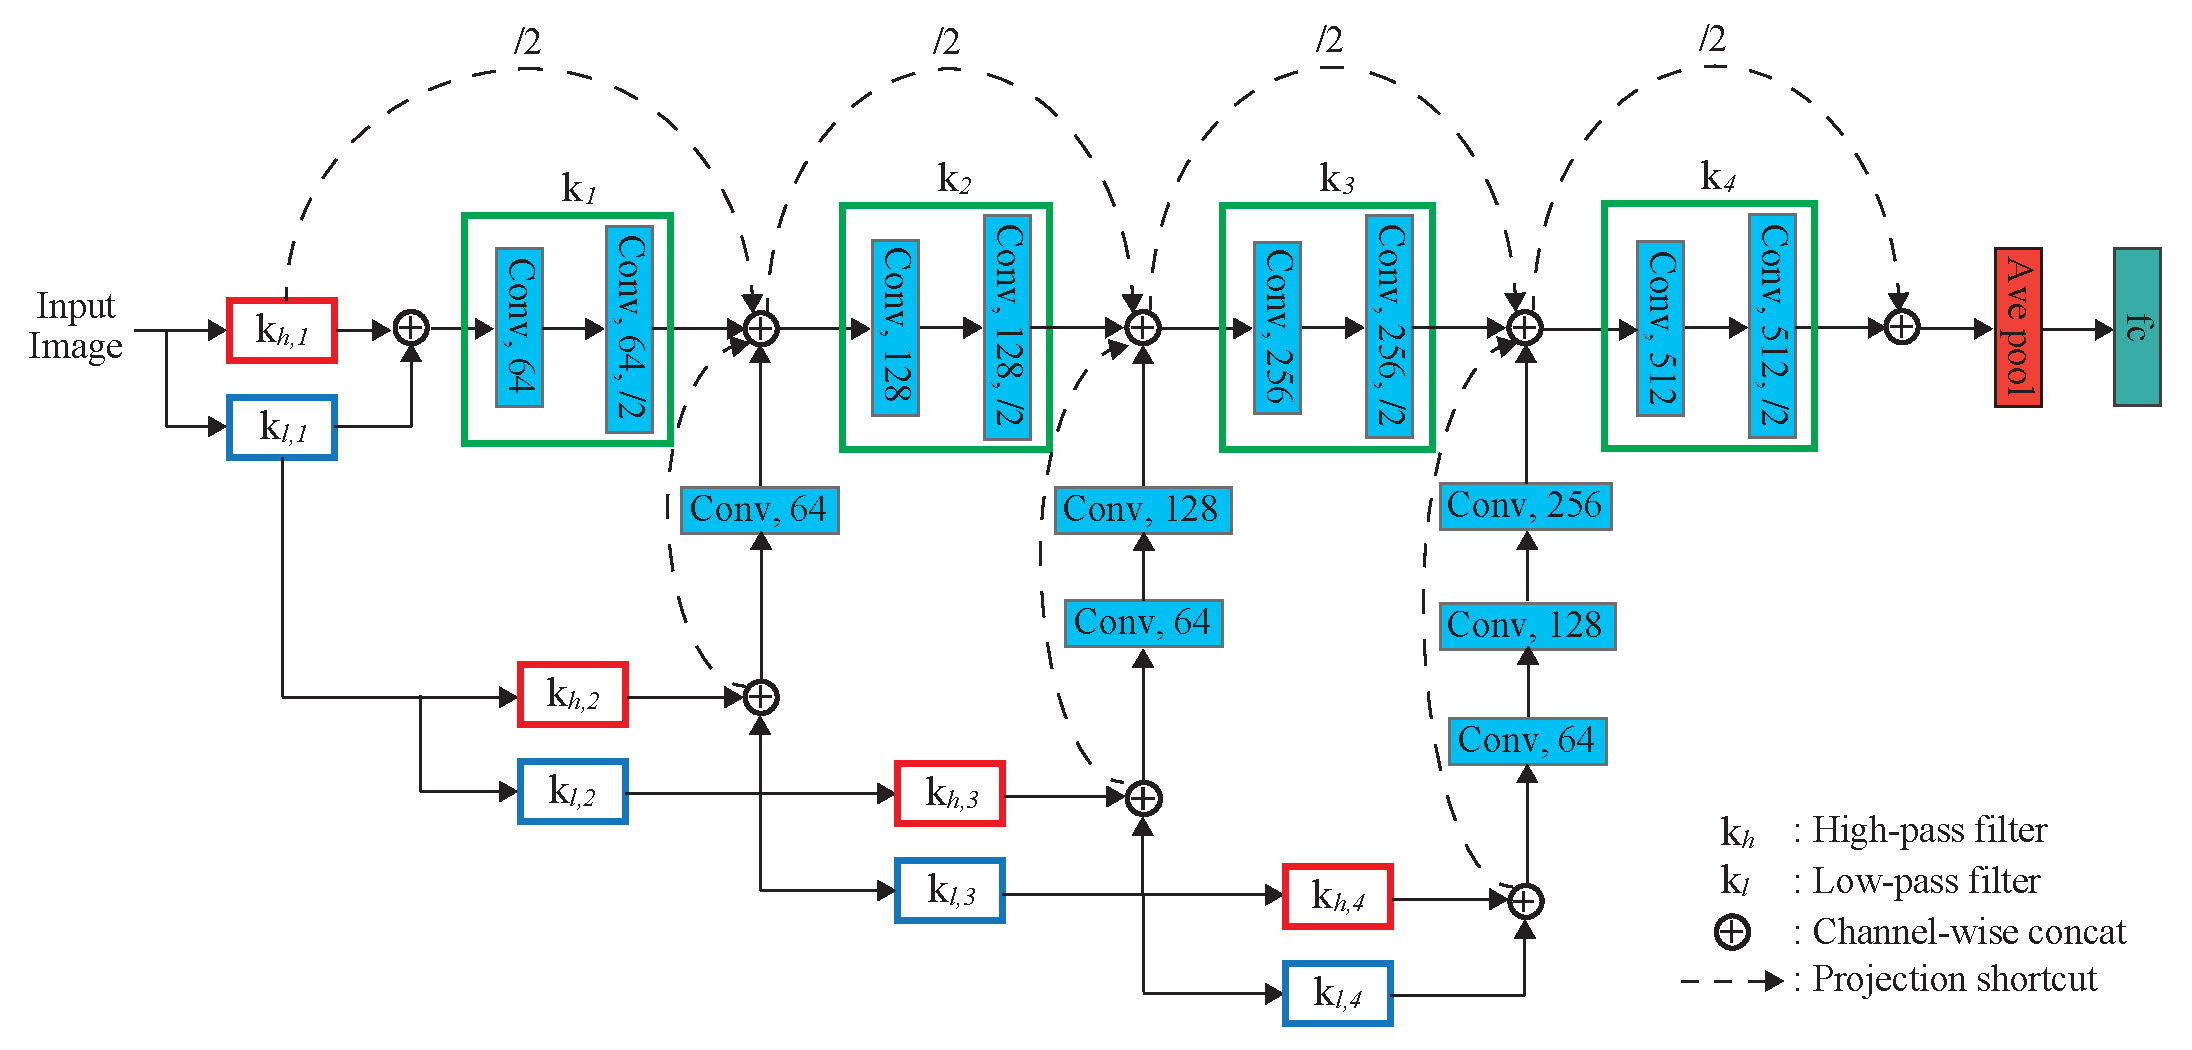
\includegraphics[width=\textwidth]{\imgpath/wavelet_CNN_3.pdf}
  \mycaption{Architecture using the DWT as a frontend to a CNN}{Figure 1 from
  \cite{fujieda_wavelet_2018}. Fujieda et.\ al.\ take a multiscale wavelet
  decomposition of the input before passing the input through a standard
  CNN\@. They learn convolutional layers independently on each subband and feed
  these back into the network at different depths, where the resolution of the
  subband and the network activations match.}
  \label{fig:ch6:fujieda}
\end{figure}

Several works also use wavelets in deep neural networks for super-resolution
\cite{guo_deep_2017} and for adding detail back into dense pixel-wise
segmentation tasks \cite{ma_detailed_2018}. These typically save wavelet
coefficients and use them for the reconstruction phase, so are a little less
applicable than the first work.


\section{Background and Notation}
We make use of the 2-D $Z$-transform to simplify our analysis:
%
\begin{equation}
  X(\zz) = \sum_{n_1}\sum_{n_2} x[n_1, n_2]z_1^{-n_1}z_2^{-n_2} =
  \sum_{\nn}x[c, \nn]\zz^{-\nn}
\end{equation}
%
As we are working with three dimensional arrays (two spatial and one channel) but are
only doing convolution in two, we introduce a slightly modified 2-D $Z$-transform
which includes the channel index:
%
\begin{equation}
  X(c, \zz) = \sum_{n_1}\sum_{n_2} x[c, n_1, n_2]z_1^{-n_1}z_2^{-n_2} =
  \sum_{\nn}x[c, \nn]\zz^{-\nn} \label{eq:ch6:ztransform}
\end{equation}
%
Recall that a typical convolutional
layer in a standard CNN gets the next layer's output in a two-step process:
%
\begin{align} 
  \cnndlact{y}{l+1}{f}{\nn} &= \sum_{c=0}^{C_l - 1} \cnndlact{x}{l}{c}{\nn} \conv \cnndfilt{l}{f}{c}{\nn}
    \label{eq:ch6:conv}\\
    \cnndlact{x}{l+1}{f}{\xy} & =  \sigma \left( \cnndlact{y}{l+1}{f}{\xy} \right) \label{eq:ch6:nonlin}
\end{align}
%
In shorthand, we can reduce the action of the convolutional layer in \eqref{eq:ch6:conv} to $\mathcal{H}$, saying:
\begin{equation}
  y^{(l+1)} = \mathcal{H}x^{(l)}
\end{equation}
%
With the new $Z$-transform notation introduced in \eqref{eq:ch6:ztransform}, we
can rewrite \eqref{eq:ch6:conv} as:
%
\begin{equation}
  \cnnlact{Y}{l+1}{f}{\zz} = \sum_{c=0}^{C_l - 1} \cnnlact{X}{l}{c}{\zz} H_f^{(l)}(c, \zz)
\end{equation}
%
Note that we cannot rewrite \eqref{eq:ch6:nonlin} with $Z$-transforms as it is a nonlinear
operation.

Also recall that with multirate systems, upsampling by $M$ takes $X(z)$ to
$X(z^M)$ and downsampling by $M$ takes $X(z)$ to $\frac{1}{M}\sum_{k=0}^{M-1} X(W_M^k
z^{1/k})$ where $W_M^k = e^{\frac{j2\pi k}{M}}$. We will drop the $M$ subscript
below unless it is unclear of the sample rate change, simply using $W^k$.

\subsection{$\DTCWT$ Notation}
For this chapter, we will work with lots of $\DTCWT$ coefficients so we define
some slightly new notation here.

A $J$ scale $\DTCWT$ gives $6J+1$ coefficients, 6 sets of complex
bandpass coefficients for each scale (representing the oriented bands from 15 to 165
degrees) and 1 set of real lowpass coefficients. 
\begin{equation}
  \DTCWT_J(x) = u_{lp}, \{u_{j,k} \}_{1\leq j\leq J, 1\leq k\leq 6}
  \label{eq:ch6:dtcwt_coeffs}
\end{equation}

Each of these coefficients then has size:
%
\begin{eqnarray}
  u_{lp} &\in & \reals[N\x C\x \frac{H}{2^{J-1}} \x \frac{W}{2^{J-1}}] \\
  u_{j,k} &\in & \complexes[N\x C\x \frac{H}{2^{J}}\x \frac{W}{2^{J}}]
\end{eqnarray}
%
Note that the lowpass coefficients are twice as large as in a fully decimated
transform, a feature of the redundancy of the $\DTCWT$.

If we ever want to refer to all the subbands at a given scale, we will
drop the $k$ subscript and call them $u_j$. Likewise, $u$ refers to the whole
set of $\DTCWT$ coefficients.

\section{Learning in Multiple Spaces}

\begin{figure}[t]
  \centering
  \includegraphics[width=0.8\textwidth]{\imgpath/fwd_chain.jpg}
  \mycaption{Proposed new forward pass in the wavelet domain}{Two network 
  layers with some possible options for processing. Solid lines denote the
  evaluation path and dashed lines indicate relationships. In (a) we see a
  regular convolutional neural network. We have included the dashed lines to
  make clear what we are denoting as $u$ and $v$ with respect to their
  equivalents $x$ and $y$. In (b) we get to $y^{(2)}$ through a different path.
  First we take the wavelet transform of $x^{(1)}$ to give $u^{(1)}$, apply a
  wavelet gain layer $\mathcal{G}^{(1)}$, and take the inverse wavelet transform
  to give $y^{(2)}$. The cross through $\mathcal{H}^{(1)}$ indicates that this
  path is no longer present. Note that there may not be any possible
  $\mathcal{G}^{(1)}$ to make $y^{(2)}$ from (b) equal $y^{(2)}$ from (a). In
  (c) we have stayed in the wavelet domain longer, and applied a wavelet
  nonlinearity $\sigma_w$ to give $u^{(2)}$. We then return to the pixel domain
  to give $x^{(2)}$ and continue on from there in the pixel domain.}
  \label{fig:ch6:fwd_chain}
\end{figure}
At the beginning of each stage of a neural network we have the activations
$x^{(l)}$. Naturally, all of these activations have their equivalent wavelet
coefficients $u^{(l)}$. 

From \eqref{eq:ch6:conv}, convolutional layers also have intermediate
activations $y^{(l)}$. Let us differentiate these from the $x$ coefficients and
modify \eqref{eq:ch6:dwt_coeffs} and \eqref{eq:ch6:dtcwt_coeffs} to say the 
$\DTCWT$ of $y^{(l)}$ gives $v$.

We now propose the wavelet gain layer $G$.
The name `gain layer' comes from the inspiration for this chapter's work, in
that the first layer of CNN could be nearly done in the wavelet domain by
setting subband gains to 0 and 1. 

The gain layer $G$ can be used instead of a convolutional layer. 
It is designed to work on the wavelet coefficients of an activation,
$u$ to give outputs $v$. 

This can be seen as breaking the convolutional path in
\autoref{fig:ch6:fwd_chain} and taking a new route to get to the next layer's
coefficients. From here, we can return to the pixel domain by taking the
corresponding inverse wavelet transform $W^{-1}$. Alternatively, we
can stay in the wavelet domain and apply a wavelet based nonlinearity $\sigma_w$
to give the next layer's $u$ coefficients. Ultimately we would like to explore
architecture design with arbitrary sections in the wavelet and pixel domain, but
to do this we must first explore: 
\begin{itemize}
  \item How effective $G$ is at replacing $H$.
  \item How effective $\sigma_w$ is at replcaing $\sigma$.
\end{itemize}

\subsection{The $\DTCWT$ Gain Layer}
To do the mixing across the $C_l$ channels at each subband, giving $C_{l+1}$
output channels, we introduce the learnable filters:
%
\begin{align}
  g_{lp} &\in \reals[C_{l+1}\x C_l\x k_{lp}\x k_{lp}] \label{eq:ch6:glp} \\
  g_{1,1} &\in \complexes[C_{l+1}\x C_l\x k_1\x k_1] \\
  g_{1,2} &\in \complexes[C_{l+1}\x C_l\x k_1\x k_1] \\
      & \vdots \nonumber \\
  g_{J,6} &\in \complexes[C_{l+1}\x C_l\x k_J\x k_J]  \label{eq:ch6:gj6}
\end{align}
%
where $k$ is the size of the mixing kernels. These could be $1\x 1$ for
simple gain control, or could be larger, say $3\x 3$, to do more complex
filtering on the subbands. 

With these gains we define $v = Gu$ to be:
\begin{align}
  v_{lp}[f, \nn] &=  \sum_{c=0}^{C_l-1} u_{lp}[c, \nn] \conv g_{lp}[f, c, \nn] \\
  v_{1,1}[f, \nn] &=  \sum_{c=0}^{C_l-1} u_{1,1}[c, \nn] \conv g_{1,1}[f, c, \nn] \\
  v_{1,2}[f, \nn] &=  \sum_{c=0}^{C_l-1} u_{1,2}[c, \nn] \conv g_{1,2}[f, c, \nn] \\
                  & \vdots \nonumber \\
  v_{J,6}[f, \nn] &=  \sum_{c=0}^{C_l-1} u_{J,6}[c, \nn] \conv g_{J,6}[f, c, \nn] 
\end{align}

Note that for complex signals $a, b$ the convolution $a \conv b$ is defined as $(a_r \conv
b_r - a_i \conv b_i) + j(a_r \conv b_i + a_i \conv b_r)$. This is shown 
in Figure~\autoref{fig:ch6:dtcwt_blk_diagram}.

\subsubsection{The Output}
Due to the shift invariant properties of the $\DTCWT$, the gain layer can achieve aliasing
cancelling and therefore has a transfer function. The proof of this is done in
\autoref{app:ch6:dtcwt}. 

\begin{figure}[ht!]
  \centering
  \def \path {misc/dtcwt_gain}
\def \imgpath {\path/images}

\section{Introduction}\label{sec:intro}

Using wavelet based methods with deep learning is nascent but not novel.
Wavelets have been applied to texture classification \cite{fujieda_wavelet_2017,
sifre_combined_2012}, super-resolution \cite{guo_deep_2017} and for adding
detail back into dense pixel-wise segmentation tasks \cite{ma_detailed_2018}.
One exciting piece of work built on wavelets is the Scattering Transform
\cite{mallat_group_2012}, which has been used as a feature extractor for
learning, firstly with simple classifiers \cite{bruna_invariant_2013,
singh_scatternet_2017}, and later as a front end to hybrid deep learning
tasks\cite{oyallon_scaling_2017, singh_scatternet_2018}. Despite their power and
simplicity, scattering features are fixed and are visibly different to regular
CNN features \cite{cotter_visualizing_2017} - their nice invariance properties
come at the cost of flexibility, as there is no ability to learn in between
scattering layers. 

For this reason, we have been investigating a slightly different approach, more
similar to the Fourier based work in \cite{rippel_spectral_2015} in which Rippel
et.\ al.\ investigate parameterization of filters in the Fourier domain. In the
forward pass, they take the inverse DFT of their filter, and then apply normal
pixel-wise convolution. We wish to extend this by not only parameterizing
filters in the wavelet domain, but by performing the convolution there as well
(i.e., also taking the activations into the wavelet domain). After processing is
done, we can return to the pixel domain. Doing these forward and inverse
transforms has two significant advantages: 

\begin{enumerate}
  \item The layers can easily replace standard convolutional layers if they
    accept and return the same format.
  \item We can learn both in the wavelet and pixel space.
\end{enumerate}

As neural network training involves presenting thousands of training samples, we
want our layer to be fast. To achieve this we would ideally choose to use a
critically sampled filter bank implementation. The fast 2-D Discrete Wavelet
Transform (DWT) is a possible option, but it has two drawbacks: it has poor
directional selectivity and any alteration of wavelet coefficients will cause
the aliasing cancelling properties of the reconstructed signal to disappear.
Instead we choose to use the Dual-Tree Complex Wavelet Transform (\DTCWT)
\cite{selesnick_dual-tree_2005} as at the expense of limited redundancy (4:1),
it enables us to have better directional selectivity, and allows us to modify
the wavelet coefficients and still have minimal aliasing terms when we
reconstruct \cite{kingsbury_complex_2001}.

\Autoref{sec:method} of the paper describes the implementation details of our design, and
\autoref{sec:results} describes the experiments and results we have done so far.

\section{Similar Work}
\subsection{Parameterizing filters in Fourier Domain}
\cite{rippel_spectral_2015} explored parameterization of filters in the DFT
domain.  Note that they do not necessarily do the convolution in the Frequency
domain, they simply parameterize a filter $\vec{w} \in \reals[F\x C\x K\x K]$ as
a set of fourier coefficients $\hat{\vec{w}} \in \complexes[F\x C\x K \x \ceil{K/2}]$
(the reduced spatial size is a result of enforcing that the inverse DFT of their
filter to be real, so the parameterization is symmetric). On the forward pass of
the neural network, they take the inverse DFT of $\hat{\vec{w}}$ to obtain
$\vec{w}$ and then convolve this with the input $\vec{x}$ as a normal CNN
would do.\footnote{The convolution may be done by taking both the image and
filter back into the fourier space but this is typically decided by the
framework, which selects the optimal convolution strategy for the filter and
input size. Note that there is not necessarily a saving to be gained by
enforcing it to do convolution by product of FFTs, as the FFT size needed for
the filter will likely be larger than $K\x K$, which would require resampling
the coefficients}.

Note that this is almost identical to a normal CNN, except it allows for
slightly a reworked filter initialization and regularization, as well as 
affecting optimizers that keep track of past updates (such as SGD with momentum, 
Adam \cite{kingma_adam:_2014} or Adagrad). \autoref{fig:rippel_spectral_figs}
shows the fourier and spatial representation of some of the filters in
\cite{rippel_spectral_2015}, as well as histograms showing the sparsity of
parameters and momenta for parameter updates. The lower mean in the distribution
of parameter momenta indicates that fewer parameters are being updated in a
constant direction.

\subsubsection{Initialization}
No specific mention is made of the initialization technique used but it may well
be helpful to put a prior over the spectra.

\subsubsection{Regularization}
Due to Parseval's theorem, it is clear that applying an L2 regularization on the
filter weights :

$$\sum_i \lnorm{w_i}{2}^2 = \sum_i \lnorm{\hat{w}_i}{2}^2 = \sum_i
  \lnorm{\real{\hat{w_i}}}{2}^2 + \lnorm{\imag{\hat{w_i}}}{2}^2 $$

However can apply L1 regularization on the complex magnitude of the DFT filter
weights to impose spectral sparsity.

\subsubsection{Optimization}
If we define the DFT as the orthonormal version, i.e. for a square image, let:

$$ U_{ab} = \frac{1}{\sqrt{N}} \exp\{ \frac{-2j\pi ab}{N} \} $$

then

\begin{align}
  Y &= \F{DFT}\{ X \} = UXU \\
  X &= \F{DFT}^{-1} \{ Y \} = U^*YU^* \\
  \Delta X &= \dydx{L}{X} = U^* \Delta Y U^* = \F{DFT}^{-1} \{\Delta Y \}\\
  \Delta Y &= \dydx{L}{Y} = U \Delta X U = \F{DFT} \{\Delta X \}
\end{align}

Parameterizing in the fourier domain does not affect linear optimizers like
vanilla SGD and SGD with momentum (including with Nesterov momentum). 
For example consider a single filter
parameterized in the DFT and spatial domains presented with the exact same data
(and for the moment with no regularization). Let the initial values for 
$\hat{\vec{w}}$ and $\vec{w}$ be:

\begin{align}
  \hat{\vec{w}}_1 &= \alpha \\
  \vec{w}_1 &= \beta = \F{DFT}^{-1}\{\alpha\} 
\end{align}

After presenting both systems with the same minibatch of samples $\mathcal{D}$
and calculating the gradient $\dydx{L}{\vec{w}}$ we update both parameters:

\begin{eqnarray*}
  \vec{w}_2 & = & \vec{w}_1 - \eta \left. \dydx{L}{\vec{w}} \right|_{\vec{w} = \beta} \\
            & = & \beta - \eta \delta_{\vec{w}}  \\
  \hat{\vec{w}}_2 & = & \hat{\vec{w}}_1 - \eta \left. \dydx{L}{\hat{\vec{w}}} \right|_{ \hat{\vec{w}} = \alpha}  \\
                  & = & \alpha - \eta \F{DFT} \{ \delta_{\vec{w}} \} 
\end{eqnarray*}

We can then compare the effect the new parameters would have on the next
minibatch by calculating $\F{DFT}^{-1} \{\hat{\vec{w}}_2 \}$:
\begin{eqnarray*}
  \F{DFT} ^{-1} \{ \hat{\vec{w}}_2 \} &=& \F{DFT} ^{-1} \left\{ \alpha - \eta \F{DFT} \{ \delta_{\vec{w}} \} \right\}  \\
       & = & \F{DFT}^{-1} \left \{ \alpha \right \} - \eta \F{DFT}^{-1} \left \{ \F{DFT} \{ \delta_{\vec{w}} \} \right \} \\
       & = & \beta - \eta \delta_{\vec{w}} \\
       & = & \vec{w}_2
\end{eqnarray*}

In fact it can easily be seen that any optimizer that uses linear combinations
of gradients makes this new parameterization identical to parameterization in
the spatial domain. Optimizers like Adam and Adagrad however have update rules
that are not simply linear combinations of past gradients and so this affects
the learning trajectory. For Adam, there is a step where the gradients are
squared to estimate the variance of the parameter updates. 

This shows that any work involving reparametrizing or rethinking filter
convolution must be careful in what is done.

Further to this, while the inspiration for the work comes from wanting to remain
in the frequency domain, it is unsatisfying to simply parameterize filters there
and then take the inverse DFT and perform normal convolution. Ideally we would
like to fully take advantage of the benefits of a frequency representation.

\begin{figure}
  \centering
  \includegraphics[width=\textwidth]{\imgpath/rippel.png}
  \mycaption{Learning Dynamics of CNNs with DFT parameterization}{(a)
  Progression over several epochs of filters parametrized in the frequency
  domain. The left column shows the parameterized filter and the right column
  its inverse DFT. (b) Sparsity patterns for different parameterizations -
  spectral representations tend to be sparser. (c) Momenta distributions for
  parameters of CNNs trained with and without spectral parameterization. In the
  spectral parameterization fewer parameters are updated.  Image taken from
  \cite{rippel_spectral_2015}.}
  \label{fig:rippel_spectral_figs}
\end{figure}


\subsection{Spectral Pooling}
The Spectral Pooling method introduced in \cite{rippel_spectral_2015} is
described in the paper as:

\begin{quote}
  We assume we are given an input $\vec{x}\in \reals[M\x N]$, and some desired
  output map dimensionality $H \x W$. First we compute the discrete Fourier
  transform of the input into the frequency domain as $y = \mathcal{F}(\vec{x})
  \in \complexes[M\x N]$, and assume that the DC componenet has been shifted to
  the center of the domain as is standard practice. We then crop the frequency
  representation by maintaining only the central $H\x W$ submatrix of
  frequencies, which we denote as $\hat{\vec{y}} \in \complexes[H\x W]$. Finally, we
  map this approximation back into the spatial domain by taking its inverse DFT
  as $\hat{\vec{x}} = \mathcal{F}^{-1}(\hat{\vec{y}}) \in \reals[H\x W]$.
\end{quote}

While they have chosen to do this in the Fourier domain, this could also be
achieved by convolving with a separable, resampled 2D sinc function of the
appropriate frequencies for the horizontal and vertical directions:

$$\hat{\vec{x}} = \frac{HW}{MN} \vec{x} \conv \F{sinc}(\frac{Hn_y}{M}) \conv
\F{sinc}(\frac{Wn_x}{N})$$

where $n_x \in \{??\}, n_y \in \{??\}$. Of course, sincs have infinite support
in the time domain, so to achieve a similar result to spectral pooling you would
have to convolve with windowed sincs, or do some other form of similar low pass
filtering with resampling. In \cite{williams_wavelet_2018} they do exactly this
and call it `wavelet pooling', which is just keeping the low-low output of a
separable 2D DWT, or simply convolving with a separable lowpass filter. They
experimentally showed that this was equivalent to spectral and average pooling.

Note that speed ups could be achieved here if the convolution is done in the
Fourier domain, as it would involve only computing the reduced spectrum size
before taking inverse DFTs.


\section{Aliasing in the DWT}
Consider a single level critically sampled DWT in 1-D. The aliasing cancelling
condition is:

$$G_0(z)H_0(-z) + G_1(z)H_1(-z) = 0$$

This is typically solved by using Quadrature Mirror Filters, i.e.

\begin{align}
  H_1(z) &= H_0(-z) \\
  G_0(z) &= H_0(z) \\
  G_1(z) &= -H_1(z) = -H_0(-z) 
\end{align}

\section{Shift Invariance of the \DTCWT}
\begin{figure}
  \includegraphics[width=\textwidth]{\imgpath/dtcwt.png}
  \mycaption{Full 1-D \DTCWT}{}
\end{figure}

\begin{figure}
  \centering
  \begin{tikzpicture}
    \matrix (m1) [minimum height=4mm, column sep=6mm, align=center]
	{
	%--------------------------------------------------------------------
		\node[coordinate]                  (m00) {};    &
		\node[coordinate]                  (m01) {};          &
		\node[dspsquare]                   (m02) {$A_a(z)$};          &
		\node[circle,draw,inner sep=1pt]   (m03) {\downsamplertext{M}}; &
		\node[dspnodeopen,dsp/label=above] (m04) {$X_a(z)$};          &
		\node[circle,draw,inner sep=1pt]   (m07) {\upsamplertext{M}}; &
		\node[dspsquare]                   (m08) {$C(z)$};          &
		\node[coordinate]                  (m09) {};          &
		\node[coordinate]                  (m0X) {};          \\
		%--------------------------------------------------------------------
		\node[dspnodefull]                 (m10) {$X(z)$};          &
		\node[coordinate]                  (m11) {};          &
		\node[coordinate]                  (m12) {};    &
		\node[coordinate]                  (m13) {};          &
		\node[coordinate]                  (m14) {};    &
		\node[coordinate]                  (m17) {};          &
		\node[coordinate]                  (m18) {};    &
		\node[dspadder]                    (m19) {};          &
		\node[]     (m1X) {};          \\
		%--------------------------------------------------------------------
		\node[coordinate]                  (m20) {};    &
		\node[coordinate]                  (m21) {};          &
		\node[dspsquare]                   (m22) {$B(z)$};          &
		\node[circle,draw,inner sep=1pt]   (m23) {\downsamplertext{M}}; &
		\node[dspnodeopen,dsp/label=below] (m24) {$X_b(z)$};          &
		\node[circle,draw,inner sep=1pt]   (m27) {\upsamplertext{M}}; &
		\node[dspsquare]                   (m28) {$D(z)$};          &
		\node[coordinate]                  (m29) {};          &
		\node[coordinate]                  (m2X) {};          \\
		%--------------------------------------------------------------------
	};
	\draw[dspline] (m10) -- (m11);
	\draw[dspline] (m11) -- (m01);
	\draw[dspline] (m11) -- (m21);
	\foreach \i in {0,2} {
    	\draw[dspconn] (m\i1) -- (m\i2);
    	\draw[dspconn] (m\i2) -- (m\i3);
    	\draw[dspline] (m\i3) -- (m\i4);
    	\draw[dspconn] (m\i4) -- (m\i7);
    	\draw[dspconn] (m\i7) -- (m\i8);
    	\draw[dspline] (m\i8) -- (m\i9);
	}
  \draw[dspconn] (m09) -- node[right] {$Y_a'(z)$} (m19);
  \draw[dspconn] (m29) -- node[right] {$Y_b'(z)$} (m19);
	\draw[dspconn] (m19) -- (m1X);
	
\end{tikzpicture}

  \mycaption{Block Diagram of 1-D \DTCWT}{Note the top and bottom paths are
  through the wavelet or scaling functions from just level m ($M=2^m$). Figure
  based on Figure~4 in \cite{kingsbury_complex_2001}.}
  \label{fig:dtcwt_two_tree}
\end{figure}

Firstly, let us look at what would happen if we retained only 1 of the subbands.
Note that we have to keep the same band from each tree. E.g. if we wanted to
keep the $x_{001}$ coefficients, we must keep $x_{001a}$ and $x_{001b}$. For any
pair of coefficients on the tree, this would look like:

e.g. if we kept $x_{001a}$ and $x_{001b}$ then $M=8$ and $A(z) =
H_{0a}(z)H_{00a}(z^2)H_{001a}(z^4)$ is the transfer fucntion from $x$ to
$x_{001a}$. The transfer functions for $B(z)$, $C(z)$ and $D(z)$ are obtained
similarly. It is well known that:

\begin{eqnarray}
  U(z) \downarrow M &\rightarrow&  U(z^M) \\
  U(z) \uparrow M &\rightarrow & \frac{1}{M}\sum_{k=0}^{M-1}U(W^kz^{1/M})
\end{eqnarray}

Where $W=e^{j2\pi/M}$. So downsampling followed by upsampling becomes:
$$U(z) \downarrow M \uparrow M \rightarrow \frac{1}{M}\sum_{k=0}^{M-1}U(W^kz)$$

This means that

  $$Y(z) = Y_{a}(z) + Y_{b}(z) = \frac{1}{M} \sum_{k=0}^{M-1} X(W^k z) [A(W^kz)C(z) + B(W^kz)D(z)]$$

The aliasing terms for which are everywhere where $k \neq 0$ (as $X(W^kz)$ is
$X(z)$ shifted by $\frac{2k\pi}{M}$). I.e. to avoid aliasing in this reduced
tree, we want to make sure that $A(W^kz)C(z) + B(W^kz)D(z) = 0$ for all $k \neq
0$.

The figure below (Fig 5 from \cite{kingsbury_complex_2001}) shows what $A(W^kz)$
and $C(z)$ look like for both the lowpass case (left) and the highpass case
(right). Note that these responses will be similar for $B(W^kz)$ and $D(z)$. For
large values of k, there is almost no overlap (i.e. 
$A(W^kz)C(z) \approx B(W^kz)D(z) \approx 0$, 
but for small values of k (particularly $k = \pm 1$),
the transition bands have significant overlap with the central response. It is
here that we need to use the flexibility of having 2 trees to ensure that
$A(W^kz)C(z)$ and $B(W^kz)D(z)$ cancel out.

\begin{figure}
  \centering
  \includegraphics[width=\textwdith]{\imgpath/overlaps.png}
\end{figure}

To do this, let us consider the lowpass filters first. If we let:

\begin{eqnarray}
  B(z) &=& z^{\pm M/2}A(z) \\
  D(z) &=& z^{\mp M/2}C(z)
\end{eqnarray}

Then

\begin{eqnarray}
  A(W^kz)C(z) + B(W^kz)D(z) &=& A(W^kz)C(z) + (W^kz)^{\pm M/2}A(W^kz) z^{\mp M/2}C(z) \\
  &=& A(W^kz)C(z) + e^{\frac{jk2\pi}{M} \times (\pm \frac{M}{2})} z^{\pm M/2} z^{\mp M/2} A(W^kz)C(z) \\
  &=& A(W^kz)C(z) + (-1)^k A(W^kz)C(z)
\end{eqnarray}

Which cancels when k is odd

Now consider the bandpass case. For shifts of $k=1$ the right half of the left peak overlaps with the left half of the right peak. For a shift of $k=2$, the left half of the left peak overlaps with the right half of the right peak. Similarly for $k=-1$ and $k=-2$. For $|k| > 2$, there is no overlap. The fact that we have overlaps at both even and odd shifts of $k$ means that we can't use the same clever trick from before. However, what we do note is that the overlap is always caused by opposite peaks (i.e. the left with the right peak, and never the left with itself, or the right with itself). The solution then is to have $B$ and $D$ have upper and lower passbands of opposite polarity, whil $A$ and $C$ should have passbands of the same polarity.

Consider two prototype complex filters $P(z)$ and $Q(z)$ each with single passbands going from $f_s/2M \rightarrow f_s/M$ (or $\frac{pi}{M} \rightarrow \frac{2*pi}{M}$) - they must be complex to have support in only one half of the frequency plane. Now say $P^*(z) = \sum_{r}p_r^*z^{-r}$ is the z-transform of the conjugate of $p_r$, which has support only in the negative half of the frequency plane. Then we can get the required filters by:

\begin{eqnarray}
A(z) &=& 2\Re [P(z)] = P(z) + P^*(z) \\
B(z) &=& 2\Im [P(z)] = -j[P(z) - P^*(z)] \\
C(z) &=& 2\Re [Q(z)] = Q(z) + Q^*(z) \\
D(z) &=& -2\Im [Q(z)] = j[Q(z) - Q^*(z)]
\end{eqnarray}

Then:
\begin{eqnarray}
A(W^kz)C(z) + B(W^kz)D(z) &=&  [P(W^kz) + P^*(W^kz)][Q(z) + Q^*(z)] + \nonumber \\
  && (-j*j)[P(W^kz) - P^*(W^kz)][Q(z) - Q^*(z)] \\
&=& P(W^kz)Q(z)[1+1] + P^*(W^kz)Q(z)[1-1] + \nonumber \\ 
  && P(W^kz)Q^*(z)[1-1] + P^*(W^kz)Q^*(z)[1+1] \\
&=& 2P(W^kz)Q(z) + 2P^*(W^kz)Q^*(z)
\end{eqnarray}

So now we only need to ensure that $P(W^kz)$ overlaps as little as possible with
$Q(z)$. This is somewhat more manageable, the diagram below shows the problem.

\begin{figure}
  \includegraphics[width=\textwidth]{\imgpath/overlaps_complex.png}
\end{figure}


\section{DTCWT Convolution}
To do full $\DTCWT$ convolution, we need to do more than the above. We don't
want to only keep some passbands, but we want to apply different gains to each
one. First, let us check that analytically this makes sense and we still won't
have aliasing when we do more general operations to the passbands. I.e. instead
of considering the above reduced tree, consider the below tree:

$$Y(z) = Y_{a}(z) + Y_{b}(z) = \frac{1}{M} \sum_{k=0}^{M-1} X(W^k z) [A(W^kz)G(W^kz^{M})C(z) + B(W^kz)H(W^kz^{M})D(z)]$$

If we set $H=G$ then we get:

$$Y(z) = Y_{a}(z) + Y_{b}(z) = \frac{1}{M} \sum_{k=0}^{M-1} X(W^k z)G(W^kz^{M}) [A(W^kz)C(z) + B(W^kz)D(z)]$$

And assuming the above analysis holds, we see that we are safe with aliasing, as
we know $[A(W^kz)C(z) + B(W^kz)D(z)] \approx 0$ for all $k\neq 0$. This means
that our equivalent filter becomes

\begin{eqnarray}
  Y(z) &=& \frac{1}{M} X(z)G(z^{M}) [A(z)C(z) + B(z)D(z)] \\
  &=& \frac{1}{M} X(z)G(z^{M}) [P(z)Q(z) + jP^{*}(z)Q^{*}(z)]
\end{eqnarray}

Now we know can assume that our $\DTCWT$ is well designed and extracts frequency
bands at local areas, then our filter $G(z^{M})$ allows us to modify these
passbands (e.g. by simply scaling if $G(z) = C$, or by more complex functions.


The output from \autoref{fig:dtcwt_two_tree} is:

$$ Y(z) = Y_a(z) + Y_b(z) = \frac{1}{M}\sum_{k=0}^{M-1} X\left(W^k z\right)
  \left[ A\left(W^kz\right)C(z) + B\left(W^kz\right)D(z) \right] $$

Where $W=e^{j2\pi/M}$.  To achieve shift invariance we need 
$A\left(W^kz\right)C(z) + B\left(W^kz\right)D(z)$ to be very small or to cancel
each other out for all $k \neq 0$.

The complex analysis filter (taking us into the wavelet domain) is 

$$P(z) = \frac{1}{2}\left(A(z)+jB(z)\right)$$

and the complex synthesis filter (returning us to the pixel domain) is 

$$Q(z) = \frac{1}{2}\left(C(z) - jD(z)\right)$$

where $A,B,C,D$ are real.  If $G(z) = G_r(z) + jG_i(z) = 1$ then the end-to-end
transfer function is (from section 4 of \cite{kingsbury_complex_2001}):

\begin{equation}\label{eq:end_to_end1}
\frac{Y(z)}{X(z)} = \frac{2}{M}\left(P(z)Q(z) + P^*(z)Q^*(z)\right)
\end{equation}

where $P, Q$ have support only in the top half of the Fourier plane and $P^*,
Q^*$ are $P$ and $Q$ reflected in the horizontal frequency axis. Examples of
$P(z)Q(z)$ for different subbands of a 2-D \DTCWT have spectra shown in
\autoref{fig:dtcwt_bands_freq}, $P^*(z)Q^*(z)$ make up the missing half of the
frequency space.\\

\section{Method}\label{sec:method}

\begin{figure}[ht]
  \centering
  \subfloat[]{%
    \includegraphics[height=6cm]{\imgpath/subbands.png}
    \label{fig:dtcwt_bands_freq}
  }
  \hspace{1cm}
%    \newline
  \subfloat[]{%
    \includegraphics[height=5.7cm]{\imgpath/impulses.png}
    \label{fig:dtcwt_bands_impulse}
  }
  \newline
  \subfloat[]{%
    \includegraphics[width=.8\textwidth]{\imgpath/examples_scale2.png}
    \label{fig:example_impulses}
  }
  \mycaption{Building blocks of the \DTCWT gain
    layer}{\subref{fig:dtcwt_bands_freq} Contour plots at -1dB and -3dB showing the
    support in the Fourier domain of the 6 subbands of the \DTCWT at scales 1
    and 2 and the scale 2 lowpass. These are the product $P(z)Q(z)$ from
    \autoref{eq:end_to_end1}.% \subref{fig:dtcwt_bands_impulse} The pixel domain
    impulse responses for the second scale wavelets.
    \subref{fig:example_impulses} Example impulses of our layer when $g_1$, and
    $g_{lp}$ are 0 and $g_2 \in \mathbb{C}^{6\x 1\x 1}$, with each real and
    imaginary element drawn from $\mathcal{N}(0,1)$. I.e., only information in
    the 6 subbands with $\frac{\pi}{4} < |w_1|, |w_2| < \frac{\pi}{2}$ from
    \subref{fig:dtcwt_bands_freq} is passed through.} 
  \label{fig:dtcwt_bands}
\end{figure}

In a standard convolutional layer, an input with $C$ channels, $H$ rows and $W$
columns is $X \in \reals[C\x H\x W]$, which is then convolved with $F$ filters
of spatial size $K$ - $w \in \reals[F \x C\x K\x K]$, giving $Y \in \reals[F\x
H\x W]$. In many systems like \cite{krizhevsky_imagenet_2012, he_deep_2015}, the
first layer is typically a selection of bandpass filters, selecting edges with
different orientations and center frequencies. In the wavelet space this would
be trivial - take a decomposition of each input channel and keep individual
subbands (or equivalently, attenuate other bands), then take the inverse wavelet
transform.  \autoref{fig:dtcwt_bands} shows the frequency space for the \DTCWT
and makes it clearer as to how this could be done practically for a two scale
transform. To attenuate all but say the $15 \degs$ band at the first scale for
the first input channel, we would need to have $13C$ gains for the 13 subbands
and $C$ input channels, $13C-1$ of which would be zero and the remaining
coefficient one.

Instead of explicitly setting the gains, we can randomly initialize them and use
backpropagation to learn what they should be. This gives us the power to learn
more complex shapes rather than simple edges, as we can mix the regions of the
frequency space per input channel in an arbitrary way. 

\subsection{Memory Cost}

Again considering a two scale transform --- instead of learning $w\in \reals[F
\x C\x K\x K]$ we learn complex gains at the two scales, and a real gain for the
real lowpass:

$$
\begin{align}
  g_1 & \in & \complexes[F\x C\x 6\x 1\x 1] \\
  g_2 &\in &\complexes[F\x C\x 6\x 1\x 1] \\
  g_{lp} &\in & \reals[F\x C\x 1\x 1]
\end{align}
$$

We have set the spatial dimension to be $1\x 1$ to show that this gain is
identical to a $1\x 1$ convolution over the complex wavelet coefficients. If we
wish, we can learn larger spatial sizes to have more complex
attenuation/magnification of the subbands. We also can use more/fewer than
2 wavelet scales.  At first glance, we have increased our parameterization by
  a factor of 25 (13 subbands, of which all but the lowpass are complex), but
each one of these gains affects a large spatial size. For the first scale, the
effective size is about $5\x 5$ pixels, for the second scale it is about $15\x
15$.

\begin{figure}[]
  \centering
  \makebox[\textwidth][c]{%
    \resizebox{1.1\textwidth}{!}{\begin{tikzpicture}
    \matrix (m1) [row sep=4mm, column sep=6mm,align=center,anchor=center]
	{
	%--------------------------------------------------------------------
		\node[coordinate]                  (m00) {};    &
		\node[coordinate]                  (m01) {};          &
		\node[dspsquare]                   (m02) {$A(z)$};          &
		\node[circle,draw,inner sep=1pt]   (m03) {\downsamplertext{M}}; &
		\node[dspnodeopen,dsp/label=above] (m04) {$V_r(z)$};          &
		\node[rectangle,draw,inner sep=2pt](m05) {$G_r(z)$}; &
		\node[dspnodeopen,dsp/label=above] (m06) {$W_r(z)$};          &
		\node[circle,draw,inner sep=1pt]   (m07) {\upsamplertext{M}}; &
		\node[dspsquare]                   (m08) {$C(z)$};          &
		\node[coordinate]                  (m09) {};          &
		\node[coordinate]                  (m0X) {};          \\
		%--------------------------------------------------------------------
		\node[dspnodefull]                 (m10) {$X(z)$};          &
		\node[coordinate]                  (m11) {};          &
		\node[coordinate]                  (m12) {};    &
		\node[coordinate]                  (m13) {};          &
		\node[coordinate]                  (m14) {};    &
		\node[coordinate]                  (m15) {};          &
		\node[coordinate]                  (m16) {};    &
		\node[coordinate]                  (m17) {};          &
		\node[coordinate]                  (m18) {};    &
		\node[dspadder]                    (m19) {};          &
		\node[label=$Y(z)$]     (m1X) {};          \\
		%--------------------------------------------------------------------
		\node[coordinate]                  (m20) {};    &
		\node[coordinate]                  (m21) {};          &
		\node[dspsquare]                   (m22) {$B(z)$};          &
		\node[circle,draw,inner sep=1pt]   (m23) {\downsamplertext{M}}; &
		\node[dspnodeopen,dsp/label=below] (m24) {$V_i(z)$};          &
		%\node[coordinate]                  (m25) {}; &
		\node[rectangle,draw,inner sep=2pt](m25) {$G_r(z)$}; &
		\node[dspnodeopen,dsp/label=below] (m26) {$W_i(z)$};          &
		\node[circle,draw,inner sep=1pt]   (m27) {\upsamplertext{M}}; &
		\node[dspsquare]                   (m28) {$D(z)$};          &
		\node[coordinate]                  (m29) {};          &
		\node[coordinate]                  (m2X) {};          \\
		%--------------------------------------------------------------------
		&&&&&&&&& \\
		&&&&&&&&& \\
		\node[coordinate]                  (m00a) {};    &
		\node[coordinate]                  (m01a) {};          &
		\node[dspsquare]                   (m02a) {$A(z^{-1})$};          &
		\node[circle,draw,inner sep=1pt]   (m03a) {\upsamplertext{M}}; &
		\node[dspnodeopen,dsp/label=above] (m04a) {$\Delta V_r(z)$};          &
		%\node[coordinate]                  (m05) {}; &
		\node[rectangle,draw,inner sep=2pt](m05a) {$G_r(z^{-1})$}; &
		\node[dspnodeopen,dsp/label=above] (m06a) {$\Delta W_r(z)$};          &
		\node[circle,draw,inner sep=1pt]   (m07a) {\downsamplertext{M}}; &
		\node[dspsquare]                   (m08a) {$C(z^{-1})$};          &
		\node[coordinate]                  (m09a) {};          &
		\node[coordinate]                  (m0Xa) {};          \\
		%--------------------------------------------------------------------
		%\node[coordinate]  (m10) {$\Delta X(z)$};          &
		\node[label=above:$\Delta X(z)$]   (m10a) {}; &
		\node[dspadder]                    (m11a) {};          &
		\node[coordinate]                  (m12a) {};    &
		\node[coordinate]                  (m13a) {};          &
		\node[coordinate]                  (m14a) {};    &
		\node[coordinate]                  (m15a) {};          &
		\node[coordinate]                  (m16a) {};    &
		\node[coordinate]                  (m17a) {};          &
		\node[coordinate]                  (m18a) {};    &
		\node[coordinate]                  (m19a) {};          &
		\node[dspnodefull]                 (m1Xa) {$\Delta Y(z)$};          \\
		%--------------------------------------------------------------------
		\node[coordinate]                  (m20a) {};    &
		\node[coordinate]                  (m21a) {};          &
		\node[dspsquare]                   (m22a) {$B(z^{-1})$};          &
		\node[circle,draw,inner sep=1pt]   (m23a) {\upsamplertext{M}}; &
		\node[dspnodeopen,dsp/label=below] (m24a) {$\Delta V_i(z)$};          &
		%\node[coordinate]                  (m25) {}; &
		\node[rectangle,draw,inner sep=2pt](m25a) {$G_r(z^{-1})$}; &
		\node[dspnodeopen,dsp/label=below] (m26a) {$\Delta W_i(z)$};          &
		\node[circle,draw,inner sep=1pt]   (m27a) {\downsamplertext{M}}; &
		\node[dspsquare]                   (m28a) {$D(z^{-1})$};          &
		\node[coordinate]                  (m29a) {};          &
		\node[coordinate]                  (m2Xa) {};          \\
		%--------------------------------------------------------------------
	};
	\draw[dspline] (m10) -- (m11);
	\draw[dspline] (m11) -- (m01);
	\draw[dspline] (m11) -- (m21);
	\foreach \i in {0,2} {
    	\draw[dspconn] (m\i1) -- (m\i2);
    	\draw[dspconn] (m\i2) -- (m\i3);
    	\draw[dspline] (m\i3) -- (m\i4);
    	\draw[dspconn] (m\i4) -- (m\i5);
    	\draw[dspline] (m\i5) -- (m\i6);
    	\draw[dspconn] (m\i6) -- (m\i7);
    	\draw[dspconn] (m\i7) -- (m\i8);
    	\draw[dspline] (m\i8) -- (m\i9);
	}
	%\draw[dspflow] (m04) --  (m06);
	%\draw[dspflow] (m24) -- (m26);
	\draw[dspconn] (m24) -- node[draw,pos=0.7,inner sep=2pt,fill=white] {$-G_i(z)$} (m06);
	\draw[dspconn] (m04) -- node[draw,pos=0.7,inner sep=2pt,fill=white] {$G_i(z)$} (m26);
	\draw[dspconn] (m09) -- (m19);
	\draw[dspconn] (m29) -- (m19);
	\draw[dspconn] (m19) -- (m1X);
	\draw[dspconn] (m11a) -- (m10a);
	\draw[dspconn] (m01a) -- (m11a);
	\draw[dspconn] (m21a) -- (m11a);
	\foreach \i in {0,2} {
    	\draw[dspconn] (m\i9a) -- (m\i8a);
    	\draw[dspconn] (m\i8a) -- (m\i7a);
    	\draw[dspline] (m\i7a) -- (m\i6a);
    	\draw[dspconn] (m\i6a) -- (m\i5a);
    	\draw[dspline] (m\i5a) -- (m\i4a);
    	\draw[dspconn] (m\i4a) -- (m\i3a);
    	\draw[dspconn] (m\i3a) -- (m\i2a);
    	\draw[dspline] (m\i2a) -- (m\i1a);
	}
	%\draw[dspflow] (m04) --  (m06);
	%\draw[dspflow] (m24) -- (m26);
	\draw[dspconn] (m06a) -- node[draw,pos=0.7,inner sep=2pt,fill=white] {$-G_i(z^{-1})$} (m24a);
	\draw[dspconn] (m26a) -- node[draw,pos=0.7,inner sep=2pt,fill=white] {$G_i(z^{-1})$} (m04a);
	\draw[dspline] (m09a) -- (m19a);
	\draw[dspline] (m29a) -- (m19a);
	\draw[dspline] (m19a) -- (m1Xa);
	
\end{tikzpicture}
}
  }
  \mycaption{Block Diagram of 1-D \DTCWT gain layer}{(Top) 
  Forward and (bottom) backward pass of our system, based on
    Figure~4 in \cite{kingsbury_complex_2001}. Ignoring the $G$ gains, the top
    and bottom paths (through $A, C$ and $B, D$ respectively) make up the the
    real and imaginary parts for \emph{one subband} of the dual tree system.
    Combined, $A+jB$ and $C-jD$ make the complex filters necessary to have
    support on one side of the Fourier domain (see \autoref{fig:dtcwt_bands}).
    Adding in the complex gain $G_r + jG_i$, we can now attenuate/shape the
    impulse response in each of the subbands. To allow for learning, we need
    backpropagation. The bottom diagram indicates how to pass gradients $\Delta
    Y(z)$ through the layer. Note that upsampling has become downsampling, and
    convolution has become convolution with the time reverse of the filter
    (represented by $z^{-1}$ terms).}
  \label{fig:fwd_bwd}
\end{figure}

\subsection{Computational Cost}

A standard convolutional layer needs $K^2 F$ multiplies per input pixel (of
which there are $C\x H\x W$). In comparison, the wavelet gain method does a set
number of operations per pixel for the forward and inverse transforms, and then
applies gains on subsampled activations. For a 2 level \DTCWT the transform
overhead is about 60 multiplies for both the forward and inverse transform. It
is important to note that unlike the filtering operation, this does not scale
with $F$. The learned gains in each subband do scale with the number of output
channels, but can have smaller spatial size (as they have larger effective
sizes) as well as having fewer pixels to operate on (because of the decimation).
The end result is that as $F$ and $C$ grow, the overhead of the $C$ forward and
$F$ inverse transforms is outweighed by cost of $FC$ mixing processes, which
should in turn be significantly less than the cost of $FC$ $K\x K$ standard
convolutions for equivalent spatial sizes.

\subsection{Examples}

\autoref{fig:example_impulses} show example impulse responses of our layer.
These impulses were generated by randomly initializing both the real and
imaginary parts of $g_2 \in \complexes[6\x 1\x 1]$ from $\mathcal{N}(0,1)$ and
$g_1, g_{lp}$ are set to 0. I.e.\ each shape has 12 random variables. It is good
to see that there is still a large degree of variability between shapes. Our
experiments have shown that the distribution of the normalized cross-correlation
between 512 of such randomly generated shapes matches the distribution for
random vectors with roughly 11.5 degrees of freedom.

\subsection{Forward propagation}

\autoref{fig:fwd_bwd} shows the block diagram using $Z$-transforms for a single
band of our system (it is based on Figure~4 in \cite{kingsbury_complex_2001}).
To keep things simple for the rest of \autoref{sec:method} the figure shown is
for a 1-D system; it is relatively straightforward to extend this to
2-D\cite{selesnick_dual-tree_2005}. %
Modifying this from the standard wavelet equations by adding the subband gains
$G_r(z)$ and $G_i(z)$, the transfer function becomes:

\begin{equation}\label{eq:end_to_end2}
  \begin{split}
    \frac{Y(z)}{X(z)} = \frac{2}{M} \left[ \right. & G_r(z^M) \left( P(z)Q(z) + P^*(z)Q^*(z) \right) +  \\ 
     & \left. jG_i(z^M) \left(P(z)Q(z)-P^*(z)Q^*(z) \right) \right]
  \end{split}
\end{equation}

\begin{table}[]
  \centering
{\renewcommand{\arraystretch}{1.2}
  \captionsetup{width=\textwidth}
  \mycaption{LeNet vs WaveLeNet results}{Comparison of LeNet with standard
    convolution to our proposed method which learns in the wavelet space
    (WaveLenet) on CIFAR-10 and CIFAR-100. Values reported are the average top-1
    accuracy (\%) rates for different train set sizes over 5 runs.}

  \begin{tabular}{cccccccc}
    \specialrule{.1em}{.1em}{.1em} 
    & Train set size & 1000 & 2000 & 5000 & 10000 & 20000 & 50000 \\ \specialrule{.1em}{.1em}{.1em} 
    \multicolumn{1}{l}{\multirow{2}{*}{CIFAR-10}} & LeNet & 
      48.5 & 52.4 & 59.5 & 65.0 & 69.5 & 73.3\\ \cline{2-8}
    \multicolumn{1}{l}{} & WaveLeNet & 
      47.3 & 52.1 & 58.7 & 63.8 & 68.0 & 72.4\\ \hline
    \multicolumn{1}{l}{\multirow{2}{*}{CIFAR-100}} & LeNet & 
      11.1 & 15.8 & 23.1 & 29.5 & 34.4 & 41.1  \\ \cline{2-8}
    \multicolumn{1}{l}{} & WaveLeNet & 
      11.1 & 15.4 & 23.2 & 28.4  & 33.9 & 39.6 \\ \specialrule{.1em}{.1em}{.1em} 
  \end{tabular}
  \label{tab:results}
}
\end{table}

\subsection{Backpropagation}

We start with the commonly known property that for a convolutional block, the
gradient with respect to the input is the gradient with respect to the output
convolved with the time reverse of the filter. More formally, if 
$Y(z) = H(z) X(z)$:

\begin{equation}\label{eq:backprop}
  \Delta X(z) = H(z^{-1}) \Delta Y(z)
\end{equation}

where $H(z^{-1})$ is the $Z$-transform of the time/space reverse of $H(z)$,
$\Delta Y(z) \triangleq \dydx{L}{Y}(z)$ is the gradient of the loss with respect
to the output, and $\Delta X(z) \triangleq \dydx{L}{X}(z)$ is the gradient of
the loss with respect to the input. If H were complex, the first term in
\autoref{eq:backprop} would be $\bar{H}(1/\bar{z})$, but as each individual
block in the \DTCWT is purely real, we can use the simpler form. 

Assume we already have access to the quantity $\Delta Y(z)$ (this is the input
to the backwards pass). \autoref{fig:bwd_pass} illustrates the backpropagation
procedure. An interesting result is that the backwards pass of an inverse
wavelet transform is equivalent to doing a forward wavelet
transform.\footnote{As shown in \autoref{fig:bwd_pass}, the analysis and
synthesis filters have to be swapped and time reversed. For orthogonal wavelet
transforms, the synthesis filters are already the time reverse of the analysis
filters, so no change has to be done. The q-shift filters of the \DTCWT
\cite{kingsbury_design_2003} have this property.} Similarly, the backwards pass
of the forward transform is equivalent to doing the inverse transform. The
weight update gradients are then calculated by finding $\Delta W(z) =
\DTCWT\left\{ \Delta Y(z) \right\}$ and then convolving with the time reverse of
the saved wavelet coefficients from the forward pass - $V(z)$.

\begin{gather}
  \Delta G_r(z) = \Delta W_r(z) V_r(z^{-1}) + \Delta W_i(z) V_i(z^{-1})  \label{eq:gr_update}\\
  \Delta G_i(z) =  -\Delta W_r(z) V_i(z^{-1}) + \Delta W_i(z) V_r(z^{-1})  \label{eq:gi_update} 
\end{gather}

Unsurprisingly, the passthrough gradients have similar form to
\autoref{eq:end_to_end2}:

\begin{equation}\label{eq:passthrough}
  \begin{split}
    \Delta X(z) = \frac{2\Delta Y(z)}{M} & \left[G_r(z^{-M})\left( PQ + P^*Q^* \right)\right. + \\
      & \left. jG_i(z^{-M}) \left(PQ-P^*Q^* \right) \right] 
\end{split}
\end{equation}

where we have dropped the $z$ terms on $P(z), Q(z), P^*(z), Q^*(z)$ for brevity.

Note that we only need to evaluate equations ~\ref{eq:gr_update},
\ref{eq:gi_update},\ref{eq:passthrough} over the support of
$G(z)$ i.e., if it is a single number we only need to calculate $\left.\Delta
G(z)\right\rvert_{z=0}$.

\section{Experiments and Preliminary Results}\label{sec:results} To examine the
effectiveness of our convolutional layer, we do a simple experiment on CIFAR-10
and CIFAR-100. For simplicity, we compare the performance using a simple yet
relatively effective convolutional architecture - LeNet
\cite{lecun_gradient-based_1998}. LeNet has 2 convolutional layers of spatial
size $5\x 5$ followed by 2 fully connected layers and a softmax final layer. We
swap both these convolutional layers out for two of our proposed wavelet gain
layers (keeping the ReLU between them). As CIFAR has very small spatial size, we
only take a single scale \DTCWT\@. Therefore each gain layer has $6$ complex
gains for the 6 subbands, and a $3\x 3$ real gain for the lowpass (a total of
$21C$ parameters vs $25C$ for the original system). We train both networks for
200 epochs with Adam \cite{kingma_adam:_2014} optimizer with a constant learning
rate of $10^{-3}$ and a weight decay of $10^{-5}$. The code is available at
\cite{cotter_dtcwt_2018}. \autoref{tab:results} shows the mean of the validation
set accuracies for 5 runs. The different columns represent undersampled training
set sizes (with 50000 being the full training set). When undersampling, we keep
the samples per class constant. We see our system perform only very slightly
worse than the standard convolutional layer. 

\section{Conclusion and Future Work}

In this work we have presented the novel idea of learning filters by taking
activations into the wavelet domain, learning mixing coefficients and then
returning to the pixel space. This work is done as a preliminary step; we
ultimately hope that learning in both the wavelet and pixel space will have many
advantages, but as yet it has not been explored. We have considered the possible
challenges this proposes and described how a multirate system can learn through
backpropagation.  

Our experiments so far have been promising. We have shown that our layer can
learn in an end-to-end system, achieving very near similar accuracies on
CIFAR-10 and CIFAR-100 to the same system with convolutional layers instead.
This is a good start and shows the plausibility of such an idea, but we need to
search for how to improve these layers if they are to be useful.  It will be
interesting to see how well we can learn on datasets with larger images - our
proposed method naturally learns large kernels, so should scale well with the
image size.

In our experiments so far, we only briefly go into the wavelet domain before
coming back to the pixel domain to do ReLU nonlinearities, however we plan to
explore using nonlinearities in the wavelet domain, such as soft-shrinkage to
denoise/sparsify the coefficients \cite{donoho_ideal_1994}. We feel there are
strong links between ReLU non-linearities and denoising/sparsity ideas, and that
there may well be useful performance gains from mixing real pixel-domain
non-linearities with complex wavelet-domain shrinkage functions. Thus we present
these ideas here as a starting point for a novel and exciting avenue of deep
network research.

  \mycaption{Block Diagram of a single channel 1-D $\DTCWT$ Gain Layer}{Here we show the real and
  imaginary trees for a single subband. Note that while it may look similar to 
  a DWT block diagram, this diagram represents the two trees for one subband rather
  than a single tree with a pair of subbands. The gain layer does a complex
  multiply, using both the real and imaginary parts of the decomposed signal.
  This preserves the shift invariance of the $\DTCWT$ for the reconstructed
  signal $Y$.
  }
  \label{fig:ch6:dtcwt_gain}
\end{figure}

For a single subband in the $\DTCWT$, the gain layer uses a complex learned
weight $g$. \autoref{fig:ch6:dtcwt_gain} shows a single subband $\DTCWT$
based gain layer. 
Let us call the low analysis filters $A = A_r + jA_i$ and 
the synthesis filters $S = S_r + jS_i$ (these are normally called $H$ and
$G$, but we keep those letters reserved for the CNN and gain layer filters). 
The output of this layer is:
\begin{equation}\label{eq:ch6:dtcwt_fwd}
  Y(z) = \frac{2}{M}X(z) \left[G_r(z^{M}) \left(A_r(z)S_r(z) + A_i(z)S_i(z)\right)
  + G_i(z^{M}) \left(A_r(z)S_i(z) - A_i(z)S_r(z)\right) \right] \\
\end{equation}
See \autoref{app:ch6:dtcwt} for the derivation. The $G_r$ term modifies the
subband gain $A_rS_r + A_iS_i$ and the $G_i$ term modifies its Hilbert Pair
$A_rS_i - A_iS_r$. \autoref{fig:ch6:dtcwt_bands} show the contour plots for the
frequency support of each of these subbands. The complex gain $g$ can be used to
reshape the frequency response for each subband independently.

\subsubsection{Backpropagation}\label{sec:ch6:dtcwt_update}
If H were complex, the first term in \autoref{eq:ch6:backprop} would be
$\bar{H}(1/\bar{z})$, but as each individual block in the $\DTCWT$ is purely
real, we can use the simpler form $H(z^{-1})$. 

Again, let us calculate $\Delta V_r(z)$ and $\Delta V_i(z)$ by backpropagating
$\Delta Y(z)$ through the inverse $\DTCWT$. Again this is the same as doing the
forward $\DTCWT$ on $\Delta Y(z)$. Then the weight update equations are:
\begin{align}
  \Delta G_r(z) &= \Delta V_r(z) U_r(z^{-1}) + \Delta V_i(z) U_i(z^{-1})  \label{eq:ch6:gr_update}\\
  \Delta G_i(z) &=  -\Delta V_r(z) U_i(z^{-1}) + \Delta V_i(z) U_r(z^{-1})  \label{eq:ch6:gi_update} 
\end{align}
%
The passthrough equations have similar form to \eqref{eq:ch6:dtcwt_fwd}:
\begin{equation}\label{eq:ch6:dtcwt_passthrough}
    \Delta X(z) = \frac{2\Delta Y(z)}{M} \left[G_r(z^{-M})\left( A_r(z)S_r(z) + A_i(z)S_i(z) \right)\right. + 
      \left. jG_i(z^{-M}) \left(A_r(z)S_i(z) - A_i(z)S_r(z) \right) \right] 
\end{equation}

\begin{figure}[t]
  \centering
  \subfloat[]{%
    \includegraphics[height=6cm]{\imgpath/subbands.png}
    \label{fig:ch6:dtcwt_bands_freq}
  }
  \hspace{1cm}
%    \newline
  \subfloat[]{%
    \includegraphics[height=5.7cm]{\imgpath/impulses.png}
    \label{fig:ch6:dtcwt_bands_impulse}
  }
  \mycaption{$\DTCWT$ subbands}{\subref{fig:ch6:dtcwt_bands_freq} -1dB and -3dB contour plots showing
  the support in the Fourier domain of the 6 subbands of the $\DTCWT$ at scales
  1 and 2, and the scale 2 lowpass. These are the product of the single side
  band filters $P(z)$ and $Q(z)$ from \autoref{thm:ch6:shiftinv}.
  \subref{fig:ch6:dtcwt_bands_impulse} The pixel domain impulse responses for
  the second scale wavelets. The Hilbert pair for each wavelet is the underlying
  sinusoid phase shifted by 90 degrees.}
  \label{fig:ch6:dtcwt_bands}
\end{figure}

\begin{figure}[t!]
  \centering
  % \subfloat[]{%
    % \resizebox{\textwidth}{!} {\begin{tikzpicture}[%
  path image/.style={%
    path picture={%
      \node at (path picture bounding box.center) {%
        \includegraphics[height=2.0cm]{#1}
      };
    }
  }, 
  path pic/.style={%
    path picture={%
      \node at (path picture bounding box.center) {%
        \includegraphics[height=0.8cm]{#1}
      };
    }
  }, 
  scale=0.6]

  \draw (8.8, 2.5, 5) node {\Large{$\mathtt{u}^{(l)}$}};
  \draw (10.0, 2.3, 5) node {\Large{$\conv$}};
  \draw (11.5, 2.45, 5) node {\Large{$\mathtt{g}^{(l)}$}};
  \draw (15, 2.5, 5) node {\Large{$\mathtt{v}^{(l+1)}$}};
  \draw (18.5, 2.5, 5) node {\Large{$\mathtt{u}^{(l+1)}$}};
  \draw (25, 0.8, 3.5) node {\Large{$x^{(l+1)}$}};
  \draw[<->] (10, -1.3, 2) -- (10, 0.5, 2) node[near end, right] {$C_{l+1}$};

  \draw (1.0, -2.5, -2) node {bandpass};
  \draw (2.0, -2.5, 12) node {lowpass};
  \draw [decorate,decoration={brace,mirror,amplitude=10pt,raise=4pt},yshift=0pt]
    (3.8,-2.5,-4) -- (4.8,-2.5,15) node [black,midway,xshift=0.8cm];
  \draw [->, fill=gray!30,ultra thick] (0.5, -2.5, 4) -- (2.5, -2.5, 4)
    node[midway, above] {$\F{DWT}$};

  \draw [decorate,decoration={brace,amplitude=10pt,raise=4pt},yshift=0pt]
    (16.5,-2.5,-4) -- (18,-2.5,15) node [black,midway,xshift=0.8cm];
  \draw [->, fill=gray!30,ultra thick] (19, -2.5, 4) -- (21.5, -2.5, 4)
    node[midway, above] {$\F{DWT}^{-1}$};
  \tikzcuboid{
  shiftx=-2.5cm,
  shifty=-2.5cm,
  shiftz=7,
  scale=0.5,
  anglex=0, 
  angley=90, 
  anglez=230,
  dimx=3, 
  dimy=3, 
  dimz=6,
  densityx=1, 
  densityy=1, 
  densityz=1,
  shade=false,
  emphedge=true,
  shadeopacity=0,
  emphstyle/.style={rounded corners=0.2pt,line width=0.3mm},
  front/.style={draw=blue!50!white,fill=blue!50!white},%
  right/.style={draw=blue!50!white,fill=blue!50!white},%
  top/.style={draw=blue!50!white,fill=blue!50!white},%
  drawxdims=true,
  dimxval=W,
  drawydims=true,
  dimyval=H,
  drawzdims=true,
  dimzval=C_l,
  }

  % Draw the 6 subband activations and their filters
  \foreach \i in {1,...,2} {
    \tikzcuboid{
    shiftx=6cm,
    shifty=-2.0cm,
    shiftz=-5+5*\i,
    scale=0.5,
    dimx=2, dimy=2, dimz=3,
    densityx=4, densityy=4, densityz=2,
    drawxdims=false,
    drawydims=false,
    dimzval=C_l,
    drawzdims=false,
    front/.style={draw=blue!50!white,fill=blue!50!white},%
    right/.style={draw=blue!50!white,fill=blue!50!white},%
    top/.style={draw=blue!50!white,fill=blue!50!white},%
    }
    \tikzcuboid{
    dimz=2,
    shiftx=12.0cm,
    }
    \tikzcuboid{
    shiftx=16.0cm,
    }
    \draw [->, fill=gray!30,ultra thick] (10+0.1*\i, -1.5, -2+2.5*\i) -- (11+0.1*\i, -1.5, -2+2.5*\i);
      % node[midway, above] {$\sigma_w$};
    \draw [->, fill=gray!30,ultra thick] (14+0.1*\i, -1.5, -2+2.5*\i) -- (15+0.1*\i, -1.5, -2+2.5*\i)
      node[midway, above] {$\sigma_w$};

    \tikzcuboid{
    shiftx=8.5cm,
    shifty=-1.0cm,
    shiftz=-5+5*\i,
    dimx=0.4, dimy=0.4, dimz=3,
    densityx=5, densityy=5, densityz=2,
    front/.style={draw=red!50!white,fill=red!50!white},%
    right/.style={draw=red!50!white,fill=red!50!white},%
    top/.style={draw=red!50!white,fill=red!50!white},%
    }
    \tikzcuboid{
    shifty=-1.5cm,
    }
    \tikzcuboid{
    shifty=-2.0cm,
    }
    \tikzcuboid{
    shifty=-2.5cm,
    }
    % \draw (8cm, -1.8cm, -15+5*\i) node {$\vdots$};
  }
  \tikzcuboid{
  shiftx=6cm,
  shifty=-2.0cm,
  shiftz=10,
  scale=0.5,
  dimx=2, dimy=2, dimz=3,
  densityx=4, densityy=4, densityz=2,
  dimxval=\frac{W}{2},
  drawxdims=true,
  dimyval=\frac{H}{2},
  drawydims=true,
  dimzval=C_l,
  drawzdims=true,
  front/.style={draw=blue!50!white,fill=blue!50!white},%
  right/.style={draw=blue!50!white,fill=blue!50!white},%
  top/.style={draw=blue!50!white,fill=blue!50!white},%
  }
  \tikzcuboid{
  shiftx=12.0cm,
  dimz=2,
  dimzval=C_{l+1},
  }
  \tikzcuboid{
  shiftx=16.0cm,
  drawxdims=false,
  drawydims=false,
  drawzdims=false
  }
  \draw [->, fill=gray!30,ultra thick] (10+3*0.1, -1.5, 5.5) -- (11+3*0.1, -1.5, 5.5);
    % node[midway, above] {$\sigma_w$};
  \draw [->, fill=gray!30,ultra thick] (14+3*0.1, -1.5, 5.5) -- (15+3*0.1, -1.5, 5.5)
      node[midway, above] {$\sigma_w$};
  \tikzcuboid{
  shiftx=8.5cm,
  shifty=-1.0cm,
  shiftz=10,
  dimx=0.4, dimy=0.4, dimz=3,
  drawxdims=false,
  drawydims=false,
  drawzdims=false,
  densityx=5, densityy=5, densityz=2,
  front/.style={draw=red!50!white,fill=red!50!white},%
  right/.style={draw=red!50!white,fill=red!50!white},%
  top/.style={draw=red!50!white,fill=red!50!white},%
  }
  \tikzcuboid{
  shifty=-1.5cm,
  }
  \tikzcuboid{
  shifty=-2.0cm,
  }
  \tikzcuboid{
  shifty=-2.5cm,
  }

  % Draw the lowpass activation and its set of filters
  \tikzcuboid{
  shiftx=6cm,
  shifty=-2.0cm,
  shiftz=30,
  scale=0.5,
  dimx=2, dimy=2, dimz=3,
  densityx=4, densityy=4, densityz=2,
  dimxval=\frac{W}{2},
  drawxdims=true,
  dimyval=\frac{H}{2},
  drawydims=true,
  dimzval=C_l,
  drawzdims=true,
  front/.style={draw=blue!50!white,fill=blue!50!white},%
  right/.style={draw=blue!50!white,fill=blue!50!white},%
  top/.style={draw=blue!50!white,fill=blue!50!white},%
  }
  \tikzcuboid{
  shiftx=12.0cm,
  dimz=2,
  drawxdims=true,
  drawydims=true,
  dimzval=C_{l+1},
  drawzdims=true
  }
  \tikzcuboid{
  shiftx=16.0cm,
  drawxdims=false,
  drawydims=false,
  drawzdims=false,
  }
  \draw [->, fill=gray!30,ultra thick] (10.5, -1.8, 14.5) -- (11.5, -1.8, 14.5);
    % node[midway, above] {$\sigma_w$};
  \draw [->, fill=gray!30,ultra thick] (14.8, -1.8, 14.5) -- (15.8, -1.8, 14.5)
    node[midway, above] {$\sigma_w$};

  \tikzcuboid{
  shiftx=8.5cm,
  shifty=-2.75cm,
  dimx=0.8, dimy=0.8, dimz=3,
  drawxdims=false,
  drawydims=false,
  drawzdims=false,
  densityx=5, densityy=5, densityz=2,
  front/.style={draw=red!50!white,fill=red!50!white},%
  right/.style={draw=red!50!white,fill=red!50!white},%
  top/.style={draw=red!50!white,fill=red!50!white},%
  }
  \tikzcuboid{
  shifty=-2.00cm,
  }
  \tikzcuboid{
  shifty=-1.25cm,
  }
  \tikzcuboid{
  shifty=-0.5cm,
  }
  \tikzcuboid{
  shiftx=23cm,
  shifty=-2.5cm,
  shiftz=7,
  scale=0.5,
  anglex=0, 
  angley=90, 
  anglez=230,
  dimx=3, 
  dimy=3, 
  dimz=6,
  densityx=1, 
  densityy=1, 
  densityz=1,
  shade=false,
  emphedge=true,
  shadeopacity=0,
  emphstyle/.style={rounded corners=0.2pt,line width=0.3mm},
  front/.style={draw=blue!50!white,fill=blue!50!white},%
  right/.style={draw=blue!50!white,fill=blue!50!white},%
  top/.style={draw=blue!50!white,fill=blue!50!white},%
  drawxdims=true,
  dimxval=W,
  drawydims=true,
  dimyval=H,
  drawzdims=true,
  dimzval=C_{l+1},
  }
  % \draw (0, .3, 0) node {\large{$x^{(l)}$}};

\end{tikzpicture}
}
    % \label{fig:ch6:dwt_blk_diagram}
  % }\newline
  % \vspace{1cm}
  % \subfloat[]{%
    % \resizebox{\textwidth}{!} {\begin{tikzpicture}[%
  path image/.style={%
    path picture={%
      \node at (path picture bounding box.center) {%
        \includegraphics[height=2.0cm]{#1}
      };
    }
  }, 
  path pic/.style={%
    path picture={%
      \node at (path picture bounding box.center) {%
        \includegraphics[height=0.8cm]{#1}
      };
    }
  }, 
  scale=0.6]
  \draw (-1, 0.8, 3.5) node {\Large{$x^{(l)}$}};
  \draw (8.5, 2.5, 0) node {\Large{$u^{(l)}$}};
  \draw (9.7, 2.3, 0) node {\Large{$\conv$}};
  \draw (11, 2.5, 0) node {\Large{$g^{(l)}$}};
  \draw (15, 2.5, 0) node {\Large{$v^{(l+1)}$}};
  \draw (18.5, 2.5, 0) node {\Large{$u^{(l+1)}$}};
  \draw (25, 0.8, 3.5) node {\Large{$x^{(l+1)}$}};
  \draw[<->] (10, -1, -2) -- (10, 0.9, -2) node[near end, right] {$C_{l+1}$};
  \tikzcuboid{
  shiftx=-2.5cm,
  shifty=-2.5cm,
  shiftz=7,
  scale=0.5,
  anglex=0, 
  angley=90, 
  anglez=230,
  dimx=3, 
  dimy=3, 
  dimz=6,
  densityx=1, 
  densityy=1, 
  densityz=1,
  shade=false,
  emphedge=true,
  shadeopacity=0,
  emphstyle/.style={rounded corners=0.2pt,line width=0.3mm},
  front/.style={draw=blue!50!white,fill=blue!50!white},%
  right/.style={draw=blue!50!white,fill=blue!50!white},%
  top/.style={draw=blue!50!white,fill=blue!50!white},%
  drawxdims=true,
  dimxval=W,
  drawydims=true,
  dimyval=H,
  drawzdims=true,
  dimzval=C_l,
  }
  \draw [decorate,decoration={brace,mirror,amplitude=10pt,raise=4pt},yshift=0pt]
    (3.8,-2.5,-8) -- (4.8,-2.5,18) node [black,midway,xshift=0.8cm];
  \draw [->, fill=gray!30,ultra thick] (0.5, -2.5, 4) -- (2.5, -2.5, 4)
    node[midway, above] {$\DTCWT$};

  % Draw the 6 subband activations and their filters
  \foreach \i in {1,...,5} {
    \tikzcuboid{
    shiftx=6cm,
    shifty=-2.0cm,
    shiftz=-15+5*\i,
    scale=0.5,
    dimx=2, dimy=2, dimz=3,
    densityx=4, densityy=4, densityz=2,
    drawxdims=false,
    drawydims=false,
    dimzval=C_l,
    drawzdims=false,
    front/.style={draw=blue!90!white,fill=blue!90!white},%
    right/.style={draw=blue!90!white,fill=blue!90!white},%
    top/.style={draw=blue!90!white,fill=blue!90!white},%
    }
    \tikzcuboid{
    dimz=2,
    shiftx=12.0cm,
    }
    \tikzcuboid{
    shiftx=16.0cm,
    }
    \draw [->, fill=gray!30,ultra thick] (9.8+0.08*\i, -1.5, -7+2.5*\i) -- (10.8+0.08*\i, -1.5, -7+2.5*\i);
      % node[midway, above] {$\sigma_w$};
    \draw [->, fill=gray!30,ultra thick] (13.8+0.08*\i, -1.5, -7+2.5*\i) -- (14.8+0.08*\i, -1.5, -7+2.5*\i)
      node[midway, above] {$\sigma_w$};

    \tikzcuboid{
    shiftx=8.5cm,
    shifty=-1.0cm,
    shiftz=-15+5*\i,
    dimx=0.4, dimy=0.4, dimz=3,
    densityx=5, densityy=5, densityz=2,
    front/.style={draw=red!90!white,fill=red!90!white},%
    right/.style={draw=red!90!white,fill=red!90!white},%
    top/.style={draw=red!90!white,fill=red!90!white},%
    }
    \tikzcuboid{
    shifty=-1.5cm,
    }
    \tikzcuboid{
    shifty=-2.0cm,
    }
    \tikzcuboid{
    shifty=-2.5cm,
    }
    % \draw (8cm, -1.8cm, -15+5*\i) node {$\vdots$};
  }
  \tikzcuboid{
  shiftx=6cm,
  shifty=-2.0cm,
  shiftz=15,
  scale=0.5,
  dimx=2, dimy=2, dimz=3,
  densityx=4, densityy=4, densityz=2,
  dimxval=\frac{W}{2},
  drawxdims=true,
  dimyval=\frac{H}{2},
  drawydims=true,
  dimzval=C_l,
  drawzdims=true,
  front/.style={draw=blue!90!white,fill=blue!90!white},%
  right/.style={draw=blue!90!white,fill=blue!90!white},%
  top/.style={draw=blue!90!white,fill=blue!90!white},%
  }
  \tikzcuboid{
  shiftx=12.0cm,
  dimz=2,
  dimzval=C_{l+1},
  }
  \tikzcuboid{
  shiftx=16.0cm,
  drawxdims=false,
  drawydims=false,
  drawzdims=false
  }
  \draw [->, fill=gray!30,ultra thick] (9.8+6*0.08, -1.5, 8) -- (10.8+6*0.08, -1.5, 8);
    % node[midway, above] {$\sigma_w$};
  \draw [->, fill=gray!30,ultra thick] (13.8+6*0.08, -1.5, 8) -- (14.8+6*0.08, -1.5, 8)
      node[midway, above] {$\sigma_w$};
  \tikzcuboid{
  shiftx=8.5cm,
  shifty=-1.0cm,
  shiftz=15,
  dimx=0.4, dimy=0.4, dimz=3,
  drawxdims=false,
  drawydims=false,
  drawzdims=false,
  densityx=5, densityy=5, densityz=2,
  front/.style={draw=red!90!white,fill=red!90!white},%
  right/.style={draw=red!90!white,fill=red!90!white},%
  top/.style={draw=red!90!white,fill=red!90!white},%
  }
  \tikzcuboid{
  shifty=-1.5cm,
  }
  \tikzcuboid{
  shifty=-2.0cm,
  }
  \tikzcuboid{
  shifty=-2.5cm,
  }

  % Draw the lowpass activation and its set of filters
  \tikzcuboid{
  shiftx=6cm,
  shifty=-2.0cm,
  shiftz=35,
  scale=0.5,
  dimx=3, dimy=3, dimz=4,
  densityx=4, densityy=4, densityz=2,
  dimxval=W,
  drawxdims=true,
  dimyval=H,
  drawydims=true,
  dimzval=C_l,
  drawzdims=true,
  front/.style={draw=blue!50!white,fill=blue!50!white},%
  right/.style={draw=blue!50!white,fill=blue!50!white},%
  top/.style={draw=blue!50!white,fill=blue!50!white},%
  }
  \tikzcuboid{
  shiftx=12.0cm,
  dimz=2,
  drawxdims=false,
  drawydims=false,
  dimzval=C_{l+1},
  drawzdims=true
  }
  \tikzcuboid{
  shiftx=16.0cm,
  drawzdims=false,
  }
  \draw [->, fill=gray!30,ultra thick] (11.+0.5, -1.5, 17.5) -- (12.0+0.5, -1.5, 17.5);
    % node[midway, above] {$\sigma_w$};
  \draw [->, fill=gray!30,ultra thick] (15.+0.5, -1.5, 17.5) -- (16.0+0.5, -1.5, 17.5)
    node[midway, above] {$\sigma_w$};

  \tikzcuboid{
  shiftx=9cm,
  shifty=-2.75cm,
  dimx=0.8, dimy=0.8, dimz=3,
  drawxdims=false,
  drawydims=false,
  drawzdims=false,
  densityx=5, densityy=5, densityz=2,
  front/.style={draw=red!50!white,fill=red!50!white},%
  right/.style={draw=red!50!white,fill=red!50!white},%
  top/.style={draw=red!50!white,fill=red!50!white},%
  }
  \tikzcuboid{
  shifty=-2.00cm,
  }
  \tikzcuboid{
  shifty=-1.25cm,
  }
  \tikzcuboid{
  shifty=-0.5cm,
  }
  \tikzcuboid{
  shiftx=23cm,
  shifty=-2.5cm,
  shiftz=7,
  scale=0.5,
  anglex=0, 
  angley=90, 
  anglez=230,
  dimx=3, 
  dimy=3, 
  dimz=6,
  densityx=1, 
  densityy=1, 
  densityz=1,
  shade=false,
  emphedge=true,
  shadeopacity=0,
  emphstyle/.style={rounded corners=0.2pt,line width=0.3mm},
  front/.style={draw=blue!50!white,fill=blue!50!white},%
  right/.style={draw=blue!50!white,fill=blue!50!white},%
  top/.style={draw=blue!50!white,fill=blue!50!white},%
  drawxdims=true,
  dimxval=W,
  drawydims=true,
  dimyval=H,
  drawzdims=true,
  dimzval=C_{l+1},
  }
  % \draw (0, .3, 0) node {\large{$x^{(l)}$}};
  \draw [decorate,decoration={brace,amplitude=10pt,raise=4pt},yshift=0pt]
    (16.5,-2.5,-8) -- (18,-2.5,18) node [black,midway,xshift=0.8cm];
  \draw [->, fill=gray!30,ultra thick] (19, -2.5, 4) -- (21.5, -2.5, 4)
    node[midway, above] {$\DTCWT^{-1}$};

\end{tikzpicture}
}
  \resizebox{\textwidth}{!}{\begin{tikzpicture}[%
  path image/.style={%
    path picture={%
      \node at (path picture bounding box.center) {%
        \includegraphics[height=2.0cm]{#1}
      };
    }
  }, 
  path pic/.style={%
    path picture={%
      \node at (path picture bounding box.center) {%
        \includegraphics[height=0.8cm]{#1}
      };
    }
  }, 
  scale=0.6]
  \draw (-1, 0.8, 3.5) node {\Large{$x^{(l)}$}};
  \draw (8.5, 2.5, 0) node {\Large{$u^{(l)}$}};
  \draw (9.7, 2.3, 0) node {\Large{$\conv$}};
  \draw (11, 2.5, 0) node {\Large{$g^{(l)}$}};
  \draw (15, 2.5, 0) node {\Large{$v^{(l+1)}$}};
  \draw (18.5, 2.5, 0) node {\Large{$u^{(l+1)}$}};
  \draw (25, 0.8, 3.5) node {\Large{$x^{(l+1)}$}};
  \draw[<->] (10, -1, -2) -- (10, 0.9, -2) node[near end, right] {$C_{l+1}$};
  \tikzcuboid{
  shiftx=-2.5cm,
  shifty=-2.5cm,
  shiftz=7,
  scale=0.5,
  anglex=0, 
  angley=90, 
  anglez=230,
  dimx=3, 
  dimy=3, 
  dimz=6,
  densityx=1, 
  densityy=1, 
  densityz=1,
  shade=false,
  emphedge=true,
  shadeopacity=0,
  emphstyle/.style={rounded corners=0.2pt,line width=0.3mm},
  front/.style={draw=blue!50!white,fill=blue!50!white},%
  right/.style={draw=blue!50!white,fill=blue!50!white},%
  top/.style={draw=blue!50!white,fill=blue!50!white},%
  drawxdims=true,
  dimxval=W,
  drawydims=true,
  dimyval=H,
  drawzdims=true,
  dimzval=C_l,
  }
  \draw [decorate,decoration={brace,mirror,amplitude=10pt,raise=4pt},yshift=0pt]
    (3.8,-2.5,-8) -- (4.8,-2.5,18) node [black,midway,xshift=0.8cm];
  \draw [->, fill=gray!30,ultra thick] (0.5, -2.5, 4) -- (2.5, -2.5, 4)
    node[midway, above] {$\DTCWT$};

  % Draw the 6 subband activations and their filters
  \foreach \i in {1,...,5} {
    \tikzcuboid{
    shiftx=6cm,
    shifty=-2.0cm,
    shiftz=-15+5*\i,
    scale=0.5,
    dimx=2, dimy=2, dimz=3,
    densityx=4, densityy=4, densityz=2,
    drawxdims=false,
    drawydims=false,
    dimzval=C_l,
    drawzdims=false,
    front/.style={draw=blue!90!white,fill=blue!90!white},%
    right/.style={draw=blue!90!white,fill=blue!90!white},%
    top/.style={draw=blue!90!white,fill=blue!90!white},%
    }
    \tikzcuboid{
    dimz=2,
    shiftx=12.0cm,
    }
    \tikzcuboid{
    shiftx=16.0cm,
    }
    \draw [->, fill=gray!30,ultra thick] (9.8+0.08*\i, -1.5, -7+2.5*\i) -- (10.8+0.08*\i, -1.5, -7+2.5*\i);
      % node[midway, above] {$\sigma_w$};
    \draw [->, fill=gray!30,ultra thick] (13.8+0.08*\i, -1.5, -7+2.5*\i) -- (14.8+0.08*\i, -1.5, -7+2.5*\i)
      node[midway, above] {$\sigma_w$};

    \tikzcuboid{
    shiftx=8.5cm,
    shifty=-1.0cm,
    shiftz=-15+5*\i,
    dimx=0.4, dimy=0.4, dimz=3,
    densityx=5, densityy=5, densityz=2,
    front/.style={draw=red!90!white,fill=red!90!white},%
    right/.style={draw=red!90!white,fill=red!90!white},%
    top/.style={draw=red!90!white,fill=red!90!white},%
    }
    \tikzcuboid{
    shifty=-1.5cm,
    }
    \tikzcuboid{
    shifty=-2.0cm,
    }
    \tikzcuboid{
    shifty=-2.5cm,
    }
    % \draw (8cm, -1.8cm, -15+5*\i) node {$\vdots$};
  }
  \tikzcuboid{
  shiftx=6cm,
  shifty=-2.0cm,
  shiftz=15,
  scale=0.5,
  dimx=2, dimy=2, dimz=3,
  densityx=4, densityy=4, densityz=2,
  dimxval=\frac{W}{2},
  drawxdims=true,
  dimyval=\frac{H}{2},
  drawydims=true,
  dimzval=C_l,
  drawzdims=true,
  front/.style={draw=blue!90!white,fill=blue!90!white},%
  right/.style={draw=blue!90!white,fill=blue!90!white},%
  top/.style={draw=blue!90!white,fill=blue!90!white},%
  }
  \tikzcuboid{
  shiftx=12.0cm,
  dimz=2,
  dimzval=C_{l+1},
  }
  \tikzcuboid{
  shiftx=16.0cm,
  drawxdims=false,
  drawydims=false,
  drawzdims=false
  }
  \draw [->, fill=gray!30,ultra thick] (9.8+6*0.08, -1.5, 8) -- (10.8+6*0.08, -1.5, 8);
    % node[midway, above] {$\sigma_w$};
  \draw [->, fill=gray!30,ultra thick] (13.8+6*0.08, -1.5, 8) -- (14.8+6*0.08, -1.5, 8)
      node[midway, above] {$\sigma_w$};
  \tikzcuboid{
  shiftx=8.5cm,
  shifty=-1.0cm,
  shiftz=15,
  dimx=0.4, dimy=0.4, dimz=3,
  drawxdims=false,
  drawydims=false,
  drawzdims=false,
  densityx=5, densityy=5, densityz=2,
  front/.style={draw=red!90!white,fill=red!90!white},%
  right/.style={draw=red!90!white,fill=red!90!white},%
  top/.style={draw=red!90!white,fill=red!90!white},%
  }
  \tikzcuboid{
  shifty=-1.5cm,
  }
  \tikzcuboid{
  shifty=-2.0cm,
  }
  \tikzcuboid{
  shifty=-2.5cm,
  }

  % Draw the lowpass activation and its set of filters
  \tikzcuboid{
  shiftx=6cm,
  shifty=-2.0cm,
  shiftz=35,
  scale=0.5,
  dimx=3, dimy=3, dimz=4,
  densityx=4, densityy=4, densityz=2,
  dimxval=W,
  drawxdims=true,
  dimyval=H,
  drawydims=true,
  dimzval=C_l,
  drawzdims=true,
  front/.style={draw=blue!50!white,fill=blue!50!white},%
  right/.style={draw=blue!50!white,fill=blue!50!white},%
  top/.style={draw=blue!50!white,fill=blue!50!white},%
  }
  \tikzcuboid{
  shiftx=12.0cm,
  dimz=2,
  drawxdims=false,
  drawydims=false,
  dimzval=C_{l+1},
  drawzdims=true
  }
  \tikzcuboid{
  shiftx=16.0cm,
  drawzdims=false,
  }
  \draw [->, fill=gray!30,ultra thick] (11.+0.5, -1.5, 17.5) -- (12.0+0.5, -1.5, 17.5);
    % node[midway, above] {$\sigma_w$};
  \draw [->, fill=gray!30,ultra thick] (15.+0.5, -1.5, 17.5) -- (16.0+0.5, -1.5, 17.5)
    node[midway, above] {$\sigma_w$};

  \tikzcuboid{
  shiftx=9cm,
  shifty=-2.75cm,
  dimx=0.8, dimy=0.8, dimz=3,
  drawxdims=false,
  drawydims=false,
  drawzdims=false,
  densityx=5, densityy=5, densityz=2,
  front/.style={draw=red!50!white,fill=red!50!white},%
  right/.style={draw=red!50!white,fill=red!50!white},%
  top/.style={draw=red!50!white,fill=red!50!white},%
  }
  \tikzcuboid{
  shifty=-2.00cm,
  }
  \tikzcuboid{
  shifty=-1.25cm,
  }
  \tikzcuboid{
  shifty=-0.5cm,
  }
  \tikzcuboid{
  shiftx=23cm,
  shifty=-2.5cm,
  shiftz=7,
  scale=0.5,
  anglex=0, 
  angley=90, 
  anglez=230,
  dimx=3, 
  dimy=3, 
  dimz=6,
  densityx=1, 
  densityy=1, 
  densityz=1,
  shade=false,
  emphedge=true,
  shadeopacity=0,
  emphstyle/.style={rounded corners=0.2pt,line width=0.3mm},
  front/.style={draw=blue!50!white,fill=blue!50!white},%
  right/.style={draw=blue!50!white,fill=blue!50!white},%
  top/.style={draw=blue!50!white,fill=blue!50!white},%
  drawxdims=true,
  dimxval=W,
  drawydims=true,
  dimyval=H,
  drawzdims=true,
  dimzval=C_{l+1},
  }
  % \draw (0, .3, 0) node {\large{$x^{(l)}$}};
  \draw [decorate,decoration={brace,amplitude=10pt,raise=4pt},yshift=0pt]
    (16.5,-2.5,-8) -- (18,-2.5,18) node [black,midway,xshift=0.8cm];
  \draw [->, fill=gray!30,ultra thick] (19, -2.5, 4) -- (21.5, -2.5, 4)
    node[midway, above] {$\DTCWT^{-1}$};

\end{tikzpicture}
}
  \label{fig:ch6:dtcwt_blk_diagram}
  \mycaption{Block diagram of proposed method to learn in the wavelet domain}{
  Activations are shaded blue and learned parameters red. The input $x^{(l)}\in
  \mathbb{R}^{C_l\x H\x W}$ is taken into the wavelet domain and each subband is
  mixed independently with $C_{l+1}$ sets of convolutional filters (this is what
  we call the \emph{wavelet gain layer}. After mixing, a possible wavelet nonlinearity 
  $\sigma_w$ is applied to the subbands, before returning to the pixel domain
  with an inverse wavelet transform.}
  \label{fig:ch6:block_diagrams}
\end{figure}

\subsection{Examples}
\autoref{fig:ch6:examples} show example impulse responses of the $\DTCWT$ gain
layer. For comparison, we also show similar `impulse responses' for a gain layer
done in the DWT domain \footnote{modifying DWT coefficients causes a loss of the
alias cancellation properties so these are not true impulse response}. The DWT 
outputs come from three random variables: a $1\x 1$ 
convolutional weight applied to each of the low-high, high-low and high-high
subbands. The $\DTCWT$ outputs come from twelve random variables. Again a $1\x
1$ convolutional weight, but now applied to six complex subbands. 
Our experiments have shown that the distribution of the normalized
cross-correlation between 512 of such randomly generated shapes for the DWT matches the
distribution for random vectors with roughly 2.8 degrees of freedom (c.f. 3
random variables in the layer). Similarly for the $\DTCWT$, the distribution of
the normalized cross-correlation matches the distribution for random vectors
with roughtly 11.5 degrees of freedom (c.f. 12 random variables in the layer).
This is particularly reassuring for the $\DTCWT$ as it is showing that there is
still representatitve power despite the redundancy of the transform.

\begin{figure}
  \centering
  \subfloat[]{%
    \includegraphics[width=\textwidth]{\imgpath/dtcwt_examples.png}
    \label{fig:ch6:dtcwt_examples}
  }
  \newline
  \subfloat[]{%
  \includegraphics[width=\textwidth]{\imgpath/dwt_examples.png}
    \label{fig:ch6:dwt_examples}
  }
  \mycaption{Example outputs from an impulse input for the proposed gain layers}{
  Example outputs $y = W^{-1}GWx$ for an impulse
  $x$ for the $\DTCWT$ gain layer and for a similarly designed DWT gain layer.
  \subref{fig:ch6:dtcwt_examples} shows the output $y$ for a $\DTCWT$ based
  system. $g_{lp} = 0$ and $g_1$ has spatial size $1\x 1$. The 12 values
  in $g_1$ are independently sampled from a random normal of variance 1.
  The 60 samples come from 60 different random draws of the weights.
  \subref{fig:ch6:dwt_examples}
  shows the outputs $y$ when $x$ is an impulse and $W$ is the DWT with a
  `db2' wavelet family. The strong horizontal and vertical properties of the DWT
  can clearly be seen in comparison to the much freer $\DTCWT$.}
  \label{fig:ch6:examples}
\end{figure}


\subsection{Implementation Details}
Before analyzing its performance, we compare the implementation properties of
our proposed layer to a standard convolutional layer.

\subsubsection{Parameter Memory Cost}\label{sec:ch6:memory}
A standard convolutional layer with $C_l$ input channels, $C_{l+1}$ output channels
and kernel size $L\x L$ has $L^2C_{l}C_{l+1}$ parameters, with $L=3$ or $L=5$
common choices for the spatial size.
\begin{equation}
  \text{\#conv params} = 9C_lC_{l+1}
\end{equation}

We must choose the spatial sizes of both the lowpass and bandpass
mixing kernels. In our work, we set the spatial support of the lowpass 
filters for the $\DTCWT$ gain layer to be $1\x 1$ and the support of the 
complex bandpass filters to be $1\x 1$.
%
Further, we typically limit ourselves initially to only considering a single scale
transform. If we wish, we can decompose the input into more scales, resulting in a larger
net area of effect. In particular, it may be useful to do a two scale transform and discard 
the first scale coefficients. This does not increase the number of gains to
learn, but changes the position of the bands in the frequency space.

This means the number of parameters is:
\begin{equation}
  \text{\#params} = (2\x 6 + 1)C_lC_{l+1} = 13C_lC_{l+1} \label{eq:ch6:memcost2}
\end{equation} 
%
This is slightly larger than the $9C_lC_{l+1}$ parameters used in a
standard $3\x 3$ convolution, but as \autoref{fig:ch6:examples} shows, the
spatial support of the full filter is larger than an equivalent one
parameterized in the filter domain. 

\subsubsection{Activation Memory Cost}\label{sec:ch6:act_memory}
A standard convolutional layer needs to save the activation $x^{(l)}$ to
convolve with the backpropagated gradient $\dydx{L}{y^{(l+1)}}$ on the backwards
pass (to give $\dydx{L}{w^{(l)}}$). For an input with $C_l$ channels of spatial
size $H\x W$, this means
%
\begin{equation}
  \text{\#conv floats} = HWC_l 
\end{equation}

Our layers require us to save the wavelet coefficients $u_{lp}$ and  $u_{j,k}$
for updating the $g$ terms as in \eqref{eq:ch6:g_update} and
\eqref{eq:ch6:gr_update}, \eqref{eq:ch6:gi_update}.  For the critically sampled
DWT, this requires:
%
\begin{equation}
  \text{\#DWT floats} = HWC_l 
\end{equation}
%
to be saved for the backwards pass. For the $4:1$ redundant $\DTCWT$, this 
requires:
%
\begin{equation}
  \text{\#$\DTCWT$ floats} = 4HWC_l 
\end{equation}
%
to be saved for the backwards pass.  You can see this difference from the
difference in the block diagrams in \autoref{fig:ch6:block_diagrams}.

Note that a single scale $\DTCWT$ gain layer requires $16/7$ times as many
floats to be saved as compared to the invariant layer of the previous chapter.
The extra cost of this comes from two things. Firstly, we keep the real and
imaginary components for the bandpass (as opposed to only the magnitude),
meaning we need $3HWC_l$ floats, rather than $\frac{3}{2}HWC_l$. Additionally,
the lowpass was downsampled in the previous chapter, requiring only
$\frac{1}{4}HWC_l$, whereas we keep the full sample rate costing $HWC_l$.

If memory is an issue and the computation of the $\DTCWT$ is very fast, then we
only need to save the $x^(l)$ coefficients and can calculate the $u$'s on the
fly during the backwards pass. Note that a two scale $\DTCWT$ gain layer would
still only require $4HWC_l$ floats.

\subsubsection{Computational Cost}\label{sec:ch6:computation}
A standard convolutional layer with kernel size $L\x L$ needs $L^2C_{l+1}$
multiplies per input pixel (of which there are $C_{l}\x H\x W$).

For the DWT with Daubechies 2 filters, the forward and inverse transform only
require about $6$ multiplies per input pixel. The mixing is then done at a
reduced spatial resolution. For our proposed kernel sizes of $3\x 3$ for the
lowpass and $1\x 1$ for the bandpass, the DWT gain layer requires:

\begin{equation}
  % \frac{7}{4}C_{l+1} + 48 \label{eq:comp}
  \text{\#DWT mults/pixel} = \underbrace{\hphantom{1} \frac{3}{4}C_{l+1} \hphantom{1}}_{\textrm{bandpass}} +
  \underbrace{\hphantom{1}\vphantom{\frac{3}{4}} \frac{3^2}{4} C_{l+1} \hphantom{1}}_{\textrm{lowpass}} + 
  \underbrace{\vphantom{\frac{3}{4}} 6}_{\text{DWT}} + 
  \underbrace{\vphantom{\frac{3}{4}} 6}_{\text{DWT}^{-1}} = \quad 4C_{l+1} + 12 \quad
  \label{eq:ch6:comp_dwt}
\end{equation}

This is smaller than a standard $3\x 3$ convolutional layer using $9C_{l+1}$
multiplies per pixel.

For the $\DTCWT$, the overhead calculations are the same as in
\autoref{sec:ch5:computation}, so we will omit their derivation here. The mixing
is however different, requiring complex convolution for the bandpass
coefficients, and convolution over a higher resolution lowpass. The bandpass has
one quarter spatial resolution at the first scale, but this is offset by the
$4:1$ cost of complex multiplies compared to real multiplies. Again assuming we
have set $J=1$ and $k_{lp} = 3$ then the total cost for the gain layer is:
%
\begin{equation}
  % \frac{7}{4}C_{l+1} + 48 \label{eq:comp}
  \text{\#$\DTCWT$ mults/pixel} = \underbrace{\hphantom{1} \frac{6\x 4}{4}C_{l+1} \hphantom{1}}_{\textrm{bandpass}} +
  \underbrace{\hphantom{1}\vphantom{\frac{6}{4}} C_{l+1} \hphantom{1}}_{\textrm{lowpass}} + 
  \underbrace{\vphantom{\frac{6}{4}} 36}_{\DTCWT} + 
  \underbrace{\vphantom{\frac{6}{4}} 36}_{\DTCWT^{-1}} = \quad 7C_{l+1} + 72 \quad
  \label{eq:ch6:comp_dtcwt}
\end{equation}
This is marginally smaller than a $3\x 3$ convolutional layer.

\subsubsection{Parameter Initialization}
For both layer types we use the Glorot Initialization scheme \cite{glorot_understanding_2010}
with $a=1$: 
%
\begin{equation}
  g_{ij} \drawnfrom U\left[ -\sqrt{\frac{6}{(C_l + C_{l+1})k^2}},\ \sqrt{\frac{6}{(C_l + C_{l+1})k^2}}\
  \right] \label{eq:ch6:glorot}
\end{equation}
where $k$ is the kernel size.
% \subsection{Forward and Backward Algorithm}
% Algorithm~\autoref{alg:ch6:inv}.
% \begin{algorithm}[tb]
\caption{Locally Invariant Convolutional Layer forward and backward
passes}\label{alg:ch6:inv}
\begin{algorithmic}[1]
\Procedure{GAINLAYERFWD}{$x,\ g_{lp},\ g_1$}
\State $u_{lp},\ u_{1} \gets \DTCWT(x^l, \mbox{nlevels}=1) $ \Comment{$u_{1}$ has 6 orientations and is complex}
  \State \textbf{save} $u_{lp},\ u_{1}$ \Comment{For the backwards pass}
  \State $v_{lp} \gets u_{lp} \conv g_{lp}$ 
  \For{$1\leq k \leq 6$}
  \State \begin{varwidth}[t]{\linewidth}  $v_{1,k} \gets 
      \left( \real{u_{1,k}} \conv \real{g_{1,k}} - \imag{u_{1,k}} \conv \imag{g_{1,k}} \right)\ +$ \par
      \hskip\algorithmicindent \hphantom{abc}$ j\left(\real{u_{1,k}} \conv \imag{g_{1,k}} + \imag{u_{1,k}} \conv \real{g_{1,k}}\right)$;
  \end{varwidth}
  \EndFor
  \State $y \gets \DTCWT^{-1}(v_{lp}, v_{1})$
  \State \textbf{return} $y$
\EndProcedure
\end{algorithmic}\vspace{10pt}
\begin{algorithmic}[1]
  \Procedure{GAINLAYERBWD}{$\dydx{L}{Y},\ g_{lp},\ g_1$}
  \State \textbf{load} $u_{lp},\ u_1$
  \State \textbf{return} $\dydx{L}{x},\ \dydx{L}{A}$
\EndProcedure
\end{algorithmic}
\end{algorithm}


